%%%%%%%%%%%%%%%%%%%%%%%%%%%%%%%%%%%%%%%%%%%%%%%%%%%%%%%%%%%%%%%%%%%%%%%%%%%%
%% Trim Size: 9.75in x 6.5in
%% Text Area: 8in (include Runningheads) x 5in
%% ws-jktr.tex   :   26-6-08
%% Tex file to use with ws-jktr.cls written in Latex2E. 
%% The content, structure, format and layout of this style file is the 
%% property of World Scientific Publishing Co. Pte. Ltd. 
%% Copyright 1995, 2002 by World Scientific Publishing Co. 
%% All rights are reserved.
%%%%%%%%%%%%%%%%%%%%%%%%%%%%%%%%%%%%%%%%%%%%%%%%%%%%%%%%%%%%%%%%%%%%%%%%%%%%
%

\documentclass{amsart}

\usepackage[pagewise]{lineno}%\linenumbers

\usepackage{amsmath,amssymb,amsthm,fullpage,mathptmx, hyperref,dsfont,framed, graphicx, subcaption, textcomp}


%%%%%%%%%%%%%%%%%% Tikz %%%%%%%%%
\usepackage{tikz}
\usetikzlibrary{shapes.geometric}
\usetikzlibrary{calc}
\usetikzlibrary{scopes}
\usetikzlibrary{decorations.markings}

\tikzset{
every picture/.style={line width=0.8pt, >=stealth,
                       baseline=-3pt,label distance=-3pt},
%%%%%%%%%%  Node styles
dotnode/.style={fill=black,circle,minimum size=2.5pt, inner sep=1pt, outer
sep=0},
morphism/.style={circle,draw,thin, inner sep=1pt, minimum size=15pt,
                 scale=0.8},
small_morphism/.style={circle,draw,thin,inner sep=1pt,
                       minimum size=10pt, scale=0.8},
coupon/.style={draw,thin, inner sep=1pt, minimum size=18pt,scale=0.8},
%%%% different line styles:
regular/.style={densely dashed},
edge/.style={thick, dashed, draw=blue, text=black},
boundary/.style={thick,  draw=blue, text=black},
overline/.style={preaction={draw,line width=2mm,white,-}},
drinfeld center/.style={>=stealth,green!60!black, double
distance=1pt,text=black},
%%%%%%% Fill styles %%%%%%%%%%%%%%%
cell/.style={fill=black!10},
subgraph/.style={fill=black!30},
%%%%%%% Mid-path arrows
midarrow/.style={postaction={decorate},
                 decoration={
                    markings,% switch on markings
                    mark=at position #1 with {\arrow{>}},
                 }},
midarrow/.default=0.5
}



\newtheorem{thm}{Theorem}[section]
%\newtheorem*{uthm}{Theorem}
\newtheorem{lem}[thm]{Lemma}
%\newtheorem*{ulem}{Lemma}
\newtheorem{prop}[thm]{Proposition}
%\newtheorem*{uprop}[thm]{Proposition}
\newtheorem{cor}[thm]{Corollary}
\newtheorem{conj}[thm]{Conjecture}
\newtheorem{defn}[thm]{Definition}
\newtheorem{rmk}[thm]{Remark}
\newtheorem{prob}[thm]{Open problem}
\newtheorem{ques}[thm]{Question}
\newtheorem{fact}[thm]{Fact}
\newtheorem{ex}[thm]{Exercise}
\newcommand{\Hs}{H}
\newcommand{\mC}{\mathcal{C}}
\newcommand{\NN}{\mathbb{N}}
\newcommand{\ZZ}{\mathbb{Z}}
% \newcommand{\lstar}{{^*}}



\DeclareMathOperator{\id}{id}
\DeclareMathOperator{\MCG}{MCG}
\DeclareMathOperator{\Mod}{Mod}
\DeclareMathOperator{\Vect}{Vec}
\DeclareMathOperator{\Homeo}{Homeo}
\DeclareMathOperator{\Hom}{Hom}
\DeclareMathOperator{\Obj}{Obj}
\DeclareMathOperator{\Irr}{Irr}
\DeclareMathOperator{\Img}{Im}
\DeclareMathOperator{\coev}{coev}
\DeclareMathOperator{\ev}{ev}
\DeclareMathOperator{\Gr}{Graph}
\DeclareMathOperator{\VGr}{VGraph}
\newcommand{\VV}{\mathbf{V}}       % boundary condition
\newcommand{\vgo}{\Vect_G^\omega}
\newcommand{\one}{1}
\newcommand{\al}{\alpha}
\newcommand{\be}{\beta}
\newcommand{\ga}{\gamma}
\newcommand{\Ga}{\Gamma}
\newcommand{\de}{\delta}
\newcommand{\De}{\Delta}
\newcommand{\ka}{\varkappa}
\newcommand{\la}{\lambda}
\newcommand{\La}{\Lambda}
\newcommand{\ph}{\varphi}
\newcommand{\Ph}{\Phi} 
\newcommand{\si}{\sigma}
\newcommand{\Si}{\Sigma}
\newcommand{\Sibar}{\overline{\Sigma}}
\newcommand{\Sihat}{\widehat{\Sigma}}
\newcommand{\om}{\omega}
\newcommand{\Om}{\Omega}
\newcommand{\eps}{\varepsilon}
\renewcommand{\th}{\theta}

%%%%%%%%%%%%%%%%%%%%%%%%%%%


\begin{document}

\markboth{Paul Gustafson}
{Finiteness of Mapping Class Group Representations from Twisted Dijkgraaf-Witten Theory}

%%%%%%%%%%%%%%%%%%%%% Publisher's Area please ignore %%%%%%%%%%%%%%
%\catchline{}{}{}{}{}
%%%%%%%%%%%%%%%%%%%%%%%%%%%%%%%%%%%%%%%%%%%%%%%%%%%%%%%%%%%%%%%%%%%

\title{Finiteness of Mapping Class Group Representations from Twisted Dijkgraaf-Witten Theory}

\author{Paul P. Gustafson}
\email{pgustafs@math.tamu.edu}
\address{Department of Mathematics,
    Texas A\&M University,
    College Station, TX
    U.S.A.}

\maketitle

\begin{abstract}
We show that any twisted Dijkgraaf-Witten representation of a mapping class group of an orientable, compact surface with boundary has finite image. This generalizes work of Etingof, Rowell and Witherspoon showing that the braid group images are finite \cite{erw}.  In particular, our result answers their question regarding finiteness of images of arbitrary mapping class group representations in the affirmative.

Our approach is to translate the problem into manipulation of colored graphs embedded in the given surface. To do this translation, we use the fact that any twisted Dijkgraaf-Witten representation associated to a finite group $G$ and 3-cocycle $\omega$ is isomorphic to a Turaev-Viro-Barrett-Westbury (TVBW) representation associated to the spherical fusion category $\Vect_G^\omega$ of twisted $G$-graded vector spaces. As shown by Kirillov, the representation space for this TVBW representation is canonically isomorphic to a vector space spanned by $\Vect_G^\omega$-colored graphs embedded in the surface \cite{kirillovStringNets}.   By analyzing the action of the Birman generators \cite{birman} on a finite spanning set of colored graphs, we find that the mapping class group acts by permutations on a slightly larger finite spanning set.  This implies that the representation has finite image.
\end{abstract}

%\keywords{TQFT; mapping class group; twisted Dijkgraaf-Witten; Property F conjecture}

%\ccode{Mathematics Subject Classification 2000: 18D10, 20F36, 57M99}

\section{Introduction}
Given a spherical fusion category $\mathcal A$ over a field $k$ and an oriented compact surface $\Si$, possibly with boundary, the Turaev-Viro-Barrett-Westbury (TVBW) construction gives a projective representation of the mapping class group $\MCG(\Si)$ \cite{hep-th/9311155, TURAEV1992865}.  A natural problem is to determine the images of such representations.  In particular, we would like to know when such a representation has finite image.

It is conjectured that any TVBW mapping class group representation associated to a spherical fusion category $\mathcal A$ has finite image if and only if  $\mathcal A$ is weakly integral.  This conjecture is a modification of the Property F conjecture \cite{erw, nr}, which states that braid group representations coming from a braided monoidal category $\mathcal C$ should have finite image if and only if $\mathcal C$ is weakly integral. Instead of only considering braid group representations, one can consider mapping class groups of arbitrary orientable surfaces.  In this case, the input categories to construct the representations must be more specialized than just braided monoidal.  One can either apply the Reshitikhin-Turaev construction to a modular tensor category, or apply the TVBW construction to a spherical fusion category.  The former is more general than the latter since the Reshitikhin-Turaev construction for the Drinfeld center $Z(\mathcal A)$ of a spherical fusion category $\mathcal A$ yields the same representation as the TVBW construction for $\mathcal A$.  However, for the case considered in this paper, the simpler TVBW construction suffices.

In this paper, our input category is  $\mathcal A = \Vect_G^\omega$, the spherical fusion category of $G$-graded vector spaces with associativity modified by a cocycle $\omega \in Z^3(G, k^\times)$.  In this case, the TVBW construction corresponds to the twisted Dijkgraaf-Witten theory of \cite{dijkgraaf1990}.  The category $\Vect_G^\omega$ is integral, so the one expects its associated mapping class group representations to have finite image.  The main contribution of this paper is to verify this for arbitrary $G$ and $\omega$.

\textbf{Acknowledgments.}  This paper would not have been written without the guidance of my advisor, Eric Rowell.  I am also grateful to Zhenghan Wang and my father Robert Gustafson for their advice.

\section{Related Work}

The closest related work is a result of Etingof, Rowell, and Witherspoon who showed purely algebraically that the braid group representations associated to the modular category $\Mod(D^\omega(G))$ have finite images \cite{erw}.   The braid group $B_n$ is the mapping class group of a disk with $n$ marked points relative to its boundary, so they asked whether their result generalizes to arbitrary mapping class group representations associated to $\Mod(D^\omega(G))$. This paper answers their question affirmatively, using a different, more geometric approach.

Prior to the current work, certain specific cases had already been solved. In the case of the torus, Ng and Schauenburg's Congruence Subgroup Theorem implies the much stronger result that any Reshitikhin-Turaev representation of the mapping class group of the torus has finite image \cite{0806.2493}.   Another related result is due to Fjelstad and Fuchs \cite{fjfu}.  They showed that, given a surface with at most one boundary component, the mapping class group representations corresponding to the untwisted (i.e. $\omega = 1$) Dijkgraaf-Witten theory have finite image.  Their paper uses an algebraic method of Lyubashenko \cite{Lyubashenko1996} that gives a projective mapping class group representation to any factorizable ribbon Hopf algebra, in their case, the double $D(G)$. In our case, we instead consider the mapping class group action on a vector space of $\Vect_G^\omega$-colored embedded graphs defined by Kirillov \cite{kirillovStringNets}, yielding a simpler, geometric proof of the more general twisted case.

Bantay also calculated the images of certain representations of mapping class groups on the Hilbert space of an orbifold model associated to $D^\omega(G)$ \cite{bantay}.  These representations appear to coincide with the twisted Dijkgraaf-Witten representations. However, due to lack of proof, the precise connection is unclear. 


\section{Background}
\subsection{The spherical fusion category $\Vect_G^\omega$}
The following definitions are well-known and can be found in, e.g., \cite{etingofTensor}.  Let $k$ be an algebraically closed field of characteristic 0,  $G$ a finite group, and $\omega \in Z^3(G, k^\times)$ a 3-cocycle.    The spherical fusion category of $G$-graded $k$-vector spaces with associativity defined by $\omega$ is denoted $\Vect_G^\omega$.  The objects of this category are vector spaces with a decomposition $V = \bigoplus_{g \in G} V_g$. Morphisms are linear maps preserving the grading. The tensor product is defined by
$$ (V \otimes W)_g = \bigoplus_{x,y \in G, xy = g} V_x \otimes W_y. $$

For each $g \in G$, pick a 1-dimensional vector space $\delta_g \in \Obj(\Vect_G^\omega)$ concentrated in degree $g$.  The set $\{\delta_g : g \in G\}$ is a complete set of pairwise non-isomorphic representatives for the isomorphism classes of simple objects of $\Vect_G^\omega$.  We will sometimes abuse notation by referring to an object $\delta_g$ by the group element $g$.  We have $\one \cong \delta_1$, and  $\delta_g^* := \delta_{g^{-1}}$ with the coevaluation and evaluation maps defined below.

For the structural morphisms,  we follow \cite{math/0601012}.  We will treat the canonical isomorphisms $\delta_g \otimes \delta_h \cong \delta_{gh}$ as identities.    The associator $\alpha_{g,h,k}:(\delta_g \otimes \delta_h) \otimes \delta_k \to \delta_g \otimes (\delta_h \otimes \delta_k)$ is defined by
$$\alpha_{g,h,k} = \omega(g,h,k) \id_{ghk}.$$ 
The evaluation $\ev_g:\delta_g^* \otimes \delta_g \to 1$ is 
$$\ev_{g} = \omega(g^{-1},g,g^{-1}) \id_1.$$  
The coevaluation $\coev_g:1 \to \delta_g \otimes \delta_g^*$ is 
$$\coev_{g} = \id_1.$$ 
The pivotal structure $j_g:\delta_g \to \delta_g^{**}$ is 
$$j_{g} = \omega(g^{-1},g,g^{-1}) \id_{g}.$$

If $\omega$ and $\omega'$ are cohomologous cocycles, then $\Vect_G^\omega$ is monoidally equivalent to $\Vect_G^{\omega'}$ \cite{etingofTensor}.  This equivalence respects the pivotal structure, so extends to an equivalence of spherical categories.  It is a basic result in group cohomology that any cocycle $\omega \in Z^3(G, k^\times)$ is cohomologous to a cocycle taking values in $\mu_{|G|}$, the roots of unity of order $|G|$.  Thus, by replacing $\Vect^\omega_G$ with an equivalent spherical category, we assume  without loss of generality that $\Img(\omega) \subset \mu_{|G|}$ (as in \cite{erw}).  

\subsection{Strictification}
The colored graph construction takes a strict pivotal category as input, so we must strictify $\Vect_G^\omega$ to get an equivalent strict pivotal monoidal $\widehat \vgo$. Every pivotal category is equivalent to a strict pivotal monoidal category by first strictifying with respect to the monoidal structure, and then strictifying with respect to the pivotal structure as follows \cite{ns}.

Given a monoidal category $\mC$, there exists a monoidally equivalent strict monoidal category $\mC'$ with objects consisting of all finite lists of objects of $\mC$ and morphisms defined by $\Hom_{\mC'}([A_1, \ldots, A_n], [B_1, \ldots, B_m]) = \Hom_\mC(((\cdots((A_1 \otimes A_2) \otimes A_3) \otimes \cdots \otimes A_n, ((\cdots((B_1 \otimes B_2) \otimes B_3) \otimes \cdots \otimes B_m)$.  The tensor product in $\mC'$ is concatenation of lists. The strictification functor applies the obvious unique composition of associators to both objects and morphisms of $\mC$, and the coherence map does the same. If $\mC$ is pivotal, this monoidal equivalence extends to an equivalence of pivotal monoidal categories (where the pivotal structure on $\mC'$ is given by applying the strictification functor to the pivotal structure of $\mC$).

Given a pivotal strict monoidal category $\mC'$, there is a strict pivotal monoidal category $\widehat \mC$ equivalent, as a pivotal monoidal category, to $\mC'$.  The objects of $\widehat \mC$ are pairs $(X, \epsilon)$ for which there exists $r \in \NN_0$ such that $X \in \mC^r$ and $\epsilon \in \ZZ_2^r$. The morphisms are
$$\Hom_{\widehat \mC}((X, \epsilon), (Y, \epsilon)) = \Hom_{\mC'}(X_1^{\epsilon_1} \otimes \cdots \otimes X_r^{\epsilon_r}, Y_1^{\epsilon_1} \otimes \cdots \otimes Y_s^{\epsilon_s}),$$
where $X^\epsilon$ is defined by $X^0 = X$ and $X^1 = X^*$. The tensor product is given by concatenation. The duality functor on $\widehat \mC$ is given by
$$(X, \epsilon)^* = ((X_r, \ldots, X_1), (\epsilon_r + 1, \ldots, \epsilon_1 + 1)).$$
The evaluation function $\ev_{(X, \epsilon)}$ on $\widehat \mC$ is inductively defined using tensor products of identities, $j_{X_i}$'s, and evaluation maps $\ev_{X_i}$ in $\mC'$, and similarly for coevaluation.  This strictification functor maps $X \in \mC'$ to $(X, 0)$ and acts on morphisms as the identity.  The coherence maps are also identity maps.

Slightly abusing notation, we will sometimes use the same symbol for both $X \in \mC$ and its images in $\mC'$ and $\widehat \mC$ under the strictification functors.

%% TODO: prove same rep for equivalent cats? move above to later section

\newcommand{\ee}{\mathbf{e}}       % oriented edge
\newcommand{\A}{\mathcal{A}}      % category 
\newcommand{\st}{\; | \;}                               %%  such that
\newcommand{\ttt}{\otimes}                              %% tensor product
\newcommand{\cc}[1]{\underset{\scriptstyle #1}{\circ}}
\newcommand{\ccc}[1]{\underset{\scriptstyle #1}{\bullet}}
\newcommand{\ti}{\tilde}
\newcommand{\ov}{\overline}
\newcommand{\del}{\partial}
\newcommand{\<}{\langle}
\renewcommand{\>}{\rangle}
\newcommand{\surjto}{\twoheadrightarrow}      %   -->> surjection
\newcommand{\injto}{\hookrightarrow}          %  (--> injection
\newcommand{\isoto}{\xrightarrow{\sim}}       % isomor.
\newcommand{\xxto}{\xrightarrow}              % long arrow
\newcommand{\firef}[1]{Figure~{\rm\ref{#1}}}
\newcommand{\R}{\mathbb{R}}       % real numbers


\subsection{Colored graphs}\label{s:colored}

The following definitions and theorem are due to Kirillov
\cite{kirillovStringNets}, and recorded here for convenience.  For any
strict pivotal spherical fusion category $\mathcal A$ and surface $\Si$,
Kirillov gives the
following presentation of the Levin-Wen model as a vector space of
colored graphs modulo local relations.  He also proves that this space
is canonically isomorphic to the TVBW vector space associated to
$\Si$.  It is straightforward to check that this isomorphism, which
amounts to replacing a triangulation with its dual graph, commutes
with the mapping class group action.


We define the functor $\A^{\boxtimes n}\to \Vect$ by
\begin{equation}\label{e:vev}
\<V_1,\dots,V_n\>=\Hom_\A(\one,
V_1\otimes\dots\otimes V_n)
\end{equation}
for any collection $V_1,\dots, V_n$ of objects of $\A$. Note that pivotal
structure gives functorial isomorphisms
\begin{equation}\label{e:cyclic}
z\colon\<V_1,\dots,V_n\>\cong \<V_n, V_1,\dots,V_{n-1}\>
\end{equation}
where
$$z(\phi)= ( \id_{V_n \otimes V_1 \otimes \cdots \otimes V_{n-1}} \otimes \ev_{V_n^*} ) \circ (\id_{V_n} \otimes \phi \otimes \id_{V_n^*} ) \circ  \coev_{V_n^*}  $$ 
and $z^n=\id$ (see \cite[Section 5.3]{BK}). Thus, up to a canonical
isomorphism, the space $\<V_1,\dots,V_n\>$ only depends on the cyclic order
of $V_1,\dots, V_n$.

We have a natural composition map 
\begin{equation}\label{e:composition}
\begin{aligned}
 \<V_1,\dots,V_n, X\> \otimes \<X^*, W_1,\dots,
W_m\> & \to\<V_1,\dots,V_n, W_1,\dots, W_m\> \\
\ph\otimes\psi & \mapsto \ph\cc{X}\psi = (\id_{V_1 \otimes \cdots \otimes V_n} \otimes \ev_{X^*} \otimes \id_{W_1 \otimes \cdots \otimes W_m}) \circ (\ph\otimes\psi).
\end{aligned}
\end{equation}


We will consider finite  graphs embedded in an oriented surface $\Si$
(which may have boundary); for such a
graph $\Ga$, let $E(\Ga)$ be the set of edges. Note that edges are not
oriented. Let $E^{or}$ be the set of oriented edges, i.e. pairs $\ee=(e,
\text{orientation of } e)$; for such an oriented edge $\ee$, we denote by
$\bar{\ee}$ the edge with opposite orientation.

If $\Si$ has a boundary, the graph is allowed to have uncolored one-valent
vertices on $\del \Si$ but no other common points with $\del \Si$; all
other  vertices will  be called interior.  We will  call the edges of $\Ga$
terminating at these  one-valent vertices {\em legs}.   
%%%%%%%%%%%%%%%%%%%%%%
\begin{defn}\label{d:coloring} Let $\Si$ be an oriented surface
(possibly with boundary) and $\Ga\subset \Si$ --- an embedded graph as
defined above.  A {\em coloring} of $\Ga$ is the
following data:

  \begin{itemize}
    \item Choice of an object $V(\ee)\in \Obj \A$ for every oriented edge
        $\ee\in E^{or}(\Ga)$ so that $V(\ov{\ee})=V(\ee)^*$.
    \item Choice of a vector $\ph(v)\in \<V(\ee_1),\dots,V(\ee_n)\>$ 
      (see \eqref{e:vev})  for    every interior vertex $v$, where 
      $\ee_1, \dots, \ee_n$ are edges incident to $v$, taken in counterclockwise 
      order and with outward orientation. % (see \firef{f:coloring}). 
\end{itemize}

An {\em isomorphism} $f$ of two colorings $\{V(\ee), \ph(v)\}$, $\{V'(\ee), \ph'(v)\}$ is a collection of isomorphisms $f_\ee \colon V(\ee)\cong 
V'(\ee)$ which  agree  with the isomorphisms $V(\ov{\ee})=V(\ee)^*$ and which 
identify $\ph', \ph$:  $\ph'(v)=f\circ\ph(v)$. 

We will denote the set of all colored graphs on a surface $\Si$ by
$\Gr(\Si)$.
\end{defn}

%%%%%%%%%%%%%%%%%%%%%%

Note that if $\Si$ has a boundary, then every colored graph $\Ga$ defines
a collection of points $B=\{b_1,\dots, b_n\}\subset \del \Si$ (the
endpoints of the legs of $\Ga$) and a collection of objects $V_b\in \Obj\
\A$ for every $b \in B$: the colors of the legs of $\Ga$ taken with
outgoing orientation. We will denote the pair $(B, \{V_b\})$ by
$\VV=\Ga\cap \del\Si$ and call it {\em boundary value}. We will denote  
$$
\Gr(\Si, \VV)=\text{set of all colored graphs in $\Si$ with boundary value
} \VV.
$$ 


We can also consider formal linear combinations of colored graphs. Namely,
for fixed boundary value $\VV$ as above, we will denote 
\begin{equation*}\label{e:vgr}
\VGr(\Si,\VV)=\{\text{formal linear combinations of graphs }\Ga\in
\Gr(\Si,\VV)\}
\end{equation*}
In particular, if $\del \Si=\varnothing$, then the only possible boundary
condition is trivial ($B=\varnothing$); in this case, we will just write
$\VGr(\Si)$. 



The following theorem is a variation of result of Reshitikhin and Turaev. 
\begin{thm}\label{t:RT}
  There is a unique  way to assign to every colored
  planar graph $\Ga$ in a disk $D\subset \R^2$ a vector
  \begin{equation*}
    \<\Ga\>_D\in \langle V(\ee_1), \dots, V(\ee_n) \rangle
  \end{equation*}
  where $\ee_1,\dots, \ee_n$ are the edges of $\Ga$ meeting the boundary
  of $D$ (legs), taken in counterclockwise order and with outgoing orientation,
  so that that following conditions are satisfied:
  \begin{enumerate}
     \item $\<\Ga\>$ only depends on the isotopy  class of $\Ga$.

    \item If $\Ga$ is a single vertex colored by
          $\ph\in \langle V(\ee_1), \dots,  V(\ee_n)\rangle$, then $\<\Ga\>=\ph$.
     
    \item Local relations shown in \firef{f:local_rels1} hold. 


\begin{figure}[ht]
%%%%%%%%%%%%%%%%%%%%%%%%%%%%%%%%%%%%%%%%%%%%%%%%%%%%%%%
%%%%%%%%%%
$$
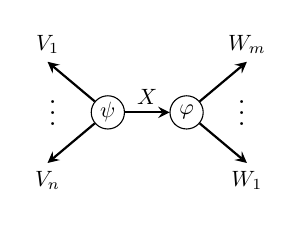
\begin{tikzpicture}
\node[morphism] (ph) at (0,0) {$\psi$};
\node[morphism] (psi) at (1,0) {$\ph$};
\node at (-0.7,0.1) {$\vdots$};
\node at (1.7,0.1) {$\vdots$};
\draw[->] (ph)-- +(220:1cm) node[pos=1.0,below,scale=0.8]
{$V_n$};
\draw[->] (ph)-- +(140:1cm) node[pos=1.0,above,scale=0.8]
{$V_1$};
\draw[->] (psi)-- +(40:1cm) node[pos=1.0,above,scale=0.8]
{$W_m$};
\draw[->] (psi)-- +(-40:1cm) node[pos=1.0,below,scale=0.8]
{$W_1$};
\draw[->] (ph) -- (psi) node[pos=0.5,above,scale=0.8] {$X$};
\end{tikzpicture}
%%%%%%%%
=
%%%%%%%%
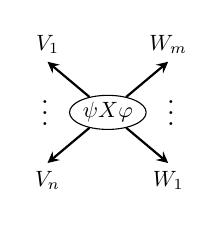
\begin{tikzpicture}
\node[ellipse, thin, scale=0.8, inner sep=1pt, draw] (ph) at (0,0)
             {$\psi\cc{X}\ph$};
\node at (-0.8,0.1) {$\vdots$};
\node at (0.8,0.1) {$\vdots$};
\draw[->] (ph)-- +(220:1cm) node[pos=1.0,below,scale=0.8] {$V_n$};
\draw[->] (ph)-- +(140:1cm) node[pos=1.0,above,scale=0.8] {$V_1$};
\draw[->] (ph)-- +(40:1cm) node[pos=1.0,above,scale=0.8]  {$W_m$};
\draw[->] (ph)-- +(-40:1cm) node[pos=1.0,below,scale=0.8] {$W_1$};
\end{tikzpicture}
%%%%%%%%%
$$
\\
$$
%%%%%%%%%
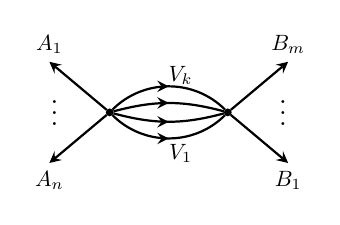
\begin{tikzpicture}
\node[dotnode] (ph) at (0,0) {};
\node[dotnode] (psi) at (1.5,0) {};
\node at (-0.7,0.1) {$\vdots$};
\node at (2.2,0.1) {$\vdots$};
\draw[->] (ph)-- +(220:1cm) node[pos=1.0,below,scale=0.8] {$A_n$};
\draw[->] (ph)-- +(140:1cm) node[pos=1.0,above,scale=0.8] {$A_1$};
\draw[->] (psi)-- +(40:1cm) node[pos=1.0,above,scale=0.8] {$B_m$};
\draw[->] (psi)-- +(-40:1cm) node[pos=1.0,below,scale=0.8] {$B_1$};
\draw[out=45,in=135, midarrow] (ph) to (psi)
                node[above,xshift=-0.6cm, yshift=0.25cm, scale=0.8] {$V_k$};
\draw[ out=15,in=165, midarrow] (ph) to (psi);
\draw[ out=-15,in=195, midarrow] (ph) to (psi);
\draw[ out=-45,in=225, midarrow] (ph) to (psi) node[below, xshift=-0.6cm, yshift=-0.3cm, scale=0.8] {$V_1$};
\end{tikzpicture}
%%%%%%%%%%%
=
%%%%%%%%%%%
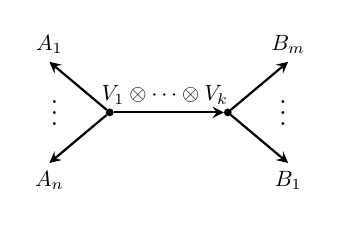
\begin{tikzpicture}
\node[dotnode] (ph) at (0,0) {};
\node[dotnode] (psi) at (1.5,0) {};
\node at (-0.7,0.1) {$\vdots$};
\node at (2.2,0.1) {$\vdots$};
\draw[->] (ph)-- +(220:1cm) node[pos=1.0,below,scale=0.8] {$A_n$};
\draw[->] (ph)-- +(140:1cm) node[pos=1.0,above,scale=0.8] {$A_1$};
\draw[->] (psi)-- +(40:1cm) node[pos=1.0,above,scale=0.8] {$B_m$};
\draw[->] (psi)-- +(-40:1cm) node[pos=1.0,below,scale=0.8] {$B_1$};
\draw[ ->] (ph) to (psi)
            node[above,xshift=-0.8cm,scale=0.8] {$V_1\otimes \dots\otimes V_k$};
\end{tikzpicture}
%%%%%%%
\qquad k\ge 0
$$
\\
$$
%%%%%%%
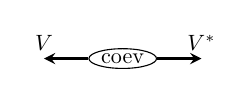
\begin{tikzpicture}
\node[ellipse, scale=0.8, inner sep=1pt, draw,thin] (ph) at (0,0)
{$\coev$};
\draw[->] (ph)-- +(180:1cm) node[pos=1.0,above,scale=0.8] {$V$};
\draw[->] (ph)-- +(0:1cm) node[pos=1.0,above,scale=0.8] {$V^*$};
\end{tikzpicture}
%%%%%%%%
=
%%%%%%%%
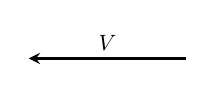
\begin{tikzpicture}
\draw[->] (2,0)-- (0,0) node[pos=0.5,above,scale=0.8] {$V$};
\end{tikzpicture}
$$
%%%%%%%%%%%%%%%%%%%%%%%%%%
\caption{Local relations for colored graphs.
%%   Here $\ph\cc{X}\psi$ denotes the morphism
%% $1 \xrightarrow{\ph \otimes \psi} 
%% V_1 \otimes \cdots \otimes V_n \otimes X \otimes X^* \otimes W_1 \otimes \cdots \otimes W_m  \xrightarrow{ev_{X^*}} 
%% V_1 \otimes \cdots \otimes V_n \otimes W_1 \otimes \cdots \otimes W_m $
%% . 
        }\label{f:local_rels1}
\end{figure}

    Local relations should be understood as follows: for any pair 
    $\Ga, \Ga'$ of colored graphs which are identical  outside a subdisk 
	$D'\subset D$, and in this disk are homeomorphic to the graphs
    shown in  \firef{f:local_rels1},  we must have $\<\Ga\>=\<\Ga'\>$. 
   \end{enumerate}

    Moreover, so defined $\<\Ga\>$ satisfies the following properties:
    \begin{enumerate} 
    \item $\<\Ga\>$ is linear in color of each vertex $v$ \textup{(}for 
         fixed colors of edges and other vertices\textup{)}.
    \item $\<\Ga\>$ is additive in colors of edges as shown in 
          \firef{f:linearity}.

\begin{figure}[ht]
$$
%%%%%%%%%%%%
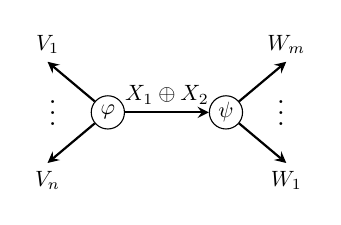
\begin{tikzpicture}
\node[morphism] (ph) at (0,0) {$\ph$};
\node[morphism] (psi) at (1.5,0) {$\psi$};
\node at (-0.7,0.1) {$\vdots$};
\node at (2.2,0.1) {$\vdots$};
\draw[->] (ph)-- +(220:1cm) node[pos=1.0,below,scale=0.8] {$V_n$};
\draw[->] (ph)-- +(140:1cm) node[pos=1.0,above,scale=0.8] {$V_1$};
\draw[->] (psi)-- +(40:1cm) node[pos=1.0,above,scale=0.8] {$W_m$};
\draw[->] (psi)-- +(-40:1cm) node[pos=1.0,below,scale=0.8] {$W_1$};
\draw[->] (ph) -- (psi) node[pos=0.5,above,scale=0.8] {$X_1\oplus X_2$};
\end{tikzpicture}
%%%%%%%%%%%%
=
%%%%%%%%%%%%
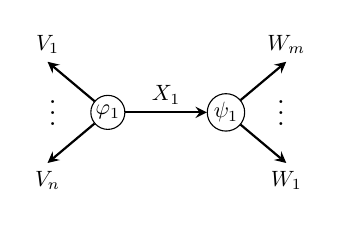
\begin{tikzpicture}
\node[morphism] (ph) at (0,0) {$\ph_1$};
\node[morphism] (psi) at (1.5,0) {$\psi_1$};
\node at (-0.7,0.1) {$\vdots$};
\node at (2.2,0.1) {$\vdots$};
\draw[->] (ph)-- +(220:1cm) node[pos=1.0,below,scale=0.8]{$V_n$};
\draw[->] (ph)-- +(140:1cm) node[pos=1.0,above,scale=0.8]{$V_1$};
\draw[->] (psi)-- +(40:1cm) node[pos=1.0,above,scale=0.8]{$W_m$};
\draw[->] (psi)-- +(-40:1cm) node[pos=1.0,below,scale=0.8]{$W_1$};
\draw[->] (ph) -- (psi) node[pos=0.5,above,scale=0.8] {$X_1$};
\end{tikzpicture}
%%%%%%%%%%%%
+
%%%%%%%%%%%%
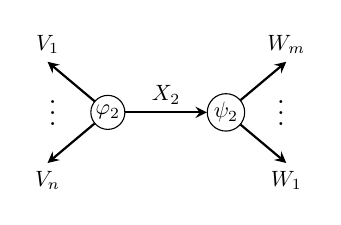
\begin{tikzpicture}
\node[morphism] (ph) at (0,0) {$\ph_2$};
\node[morphism] (psi) at (1.5,0) {$\psi_2$};
\node at (-0.7,0.1) {$\vdots$};
\node at (2.2,0.1) {$\vdots$};
\draw[->] (ph)-- +(220:1cm) node[pos=1.0,below,scale=0.8]{$V_n$};
\draw[->] (ph)-- +(140:1cm) node[pos=1.0,above,scale=0.8]{$V_1$};
\draw[->] (psi)-- +(40:1cm) node[pos=1.0,above,scale=0.8]{$W_m$};
\draw[->] (psi)-- +(-40:1cm) node[pos=1.0,below,scale=0.8]{$W_1$};
\draw[->] (ph) -- (psi) node[pos=0.5,above,scale=0.8] {$X_2$};
\end{tikzpicture}
%%%%%%%%%%%%
$$
\caption{Linearity of $\<\Ga\>$. Here $\ph_1,\ph_2$ are compositions
of $\ph$ with projector $X_1\oplus X_2\to X_1$ (respectively, 
$X_1\oplus X_2\to X_2$), and similarly for $\psi_1,\psi_2$.
}\label{f:linearity}
\end{figure}
    \item If $\Ga,\Ga'$ are two isomorphic colorings of the same graph,
      then $\<\Ga\>=\<\Ga'\>$. 
    
    \item Composition property: if $D'\subset D$ is a subdisk such
      that $\del D'$ does not contain vertices of $\Ga$ and meets edges of
      $\Ga$ transversally, then   $\<\Ga\>_D$ will not change if we replace
      subgraph $\Ga\cap D'$ by a single vertex colored by
      $\<\Ga\cap D'\>_{D'}$.

  \end{enumerate}
The vector $\<\Ga\>$ is called the {\em evaluation} of $\Ga$.
\end{thm}

To define local relations between embedded graphs, Kirillov defines the space of null graphs as follows. Let
$\Ga=c_1\Ga_1+\dots+c_n\Ga_n$ be a formal linear
combination of colored graphs in $\Si$.  If there exists an embedded disk $D \subset M$ such that
\begin{enumerate}
  \item $\Ga$ is transversal to $\del D$ (i.e., no vertices of $\Ga_i$ 
      are on the boundary of $D$ and edges of each $\Ga_i$ meet 
      $\del D$ transversally),
  \item all $\Ga_i$ coincide outside of $D$,
  \item and $\<\Ga\>_D=\sum c_i\<\Ga_i\cap D\>_D=0$;
\end{enumerate}
then $\Ga$ is called a null graph. 




\begin{defn}
The vector space $H := \Hs(\Si, \VV)$ associated to a oriented surface $\Si$ with boundary condition $\VV$ by the spherical fusion category $\mathcal A$ is the quotient space
 $$
   \Hs(\Si, \VV)=\VGr(\Si, \VV)/N(\Si, \VV)
  $$
  where $N(\Si, \VV)$ is  the subspace spanned by null graphs 
  (for all possible embedded disks  $D \subset \Si$). 
\end{defn}
%% The action of the mapping class group on H

\section{Results}


%% \begin{prop}
%% The action of the mapping class group on the vector space $H$ induced by the action of the orientation-preserving homeomorphisms on the surface $\Si$ is well-defined.
%% \end{prop}
%% \begin{proof}
%% The orientation-preserving group $\Homeo^+(M)$ acts on colored embedded graphs in $\Si$.  To see that the mapping class group $\MCG(\Si)$ has a well-defined action on $H$, we need to check two things: first, that isotopic homeomorphisms acting on a colored graph take it to equivalent colored graphs and, second, that a homeomorphism maps equivalent colored graphs to equivalent colored graphs.

%% For the first, suppose $f, g \in Homeo^+(M)$ are isotopic, with $H: M \times I \to M$ an isotopy from $f$ to $g$.  Let $i: \Gamma \to M$ be an graph embedding.  Then $H \circ i$ is an isotopy from $f \circ i$ to $g \circ i$.    

%% For the second,  to check that a homeomorphism $f \in \Homeo^+(M)$ preserves equivalence of colored graphs, it suffices to check that it in the case of each local move.  Since the mapping class group is generated by Dehn twists, all the local moves reduce to the isotopy move. 

%% To check that isotopic colored graphs get mapped to equivalent colored graphs, suppose $\Gamma$ is a graph and $i: \Gamma to M$ and $j: \Gamma \to M$ are isotopic embeddings. Let $H: \Gamma \times I \to M$ be an isotopy from $i$ to $j$.  Let $f \in \Homeo^+(M)$.  Then $f \circ H$ is an isotopy from $f \circ i$ to $f \circ j$.  

%% Thus, the action of the mapping class group on $H$ is well-defined.
%% \end{proof}

%% TODO: Prove that the Turaev-Viro/ RT construction gives the same thing for equivalent TQFTs

\newcommand{\B}{\mathcal B}

%% \begin{prop} \label{prop:equivCats}
%% Let $\Sigma$ be a compact surface with boundary. Let $\mathcal A$ and $\mathcal B$ be monoidally equivalent spherical fusion categories.  Then
%% the TVBW-representation $\rho_A : \MCG(\Sigma) \to GL(H_A)$ associated to $\mathcal A$ is isomorphic to the representation associated to $\mathcal B$.
%% \end{prop}
%% \begin{proof}
%% Let $(F, J)$ be a monoidal equivalence from $\A$ to $\B$. I claim that $F$ induces an isomorphism $\overline{F}: H_A \to H_B$ by acting on the labels.  To see that this is well-defined, we need to check that if $\phi \in \Hom(\one, V_1 \otimes \cdot \otimes V_n)$ then $F(\phi) \in    \Hom(\one, F(V_1) \otimes \cdot \otimes F(V_n))$


%% To see this, we need to check that $F$ preserves the local relations.  For the first local relation (contracting an edge), we need to check that $F(\ev_{F(X)}) \circ (F(\phi) \otimes F(\psi)) = F(\ev_{F(X)} \circ (\phi \otimes \psi))$.
%% \end{proof}


To show that the image of any $\Vect_G^\omega$ mapping class group representation is finite, we will analyze the action of the mapping class group on a finite collection of colored graphs that span the representation space $H$.  To define this spanning set, we will need the following definitions of simple morphisms and colored graphs.


\begin{defn} \label{def:simple_morphism}
Let $g_1, \ldots, g_n \in G$ and $\epsilon_1, \ldots, \epsilon_n  \in \{\pm 1\} = \ZZ_2$.  A morphism $\phi \in \langle (\delta_{g_1}, \epsilon_1), \ldots, (\delta_{g_n}, \epsilon_n) \rangle = \Hom_{\widehat{\vgo}}(1, (\delta_{g_1}, \epsilon_1) \otimes \cdots \otimes (\delta_{g_n}, \epsilon_n)) = \Hom_{\vgo}(1, (( \cdots (\delta_{g_1^{\epsilon_1}} \otimes \delta_{g_2^{\epsilon_2}}) \otimes \cdots  \otimes \delta_{g_n^{\epsilon_n}})$ will be called \emph{nice} if it is the composition of the isomorphism $\one \cong \delta_1$ and  tensor product isomorphisms of the form $\delta_{gh} \cong \delta_g \otimes \delta_h$ in $\vgo$.
\end{defn}

By MacLane's coherence theorem applied to the $\vgo$ Hom-space, there is a unique simple morphism in $\langle (\delta_{g_1}, \epsilon_1), \ldots, (\delta_{g_n}, \epsilon_n) \rangle$ whenever $\prod_{i=1}^n g_i = 1$. This simple morphism is a canonical basis element for the 1-dimensional space $\langle (\delta_{g_1}, \epsilon_1), \ldots, (\delta_{g_n}, \epsilon_n) \rangle$.  We will describe a map between such spaces as multiplication by a scalar, where the scalar is the matrix coefficient of the map with respect to these canonical bases.

\begin{defn} \label{def:simple_graph}
Let $\Gamma$ be a graph embedded in a surface $\Si$.  A $\widehat {\Vect_G^\omega}$-coloring $(V, \phi)$ of $\Gamma$ will be called \emph{simple} if the following conditions both hold: 
\begin{enumerate}
\item For every oriented edge $\ee \in E^{or}(\Gamma)$, there exists a group element $g(\ee) \in G$ and $\epsilon(\ee) \in \{\pm 1\} = \ZZ_2$ such that the coloring $V(\ee) = (\delta_{g(\ee)}, \epsilon(\ee)),$.
\item If $v$ is an interior vertex of $\Gamma$, then there exists an enumeration  $\ee_1, \dots, \ee_n$ of the edges incident to $v$, taken in counterclockwise order and with outward orientation, such that $\prod_{i=1}^n g(\ee_i)^{\epsilon(\ee_i)} = 1$ and  the vertex label $\phi(v) \in \langle g(\ee_1), \ldots, g(\ee_n) \rangle$ is a simple morphism.
\end{enumerate}
\end{defn}


\begin{lem} \label{lem:z_simple}
Let $\phi \in \langle (g_1, \epsilon_1), \ldots, (g_n, \epsilon_n) \rangle$ and $\psi \in \langle (g_n, \epsilon_n), (g_1, \epsilon_1), \ldots, (g_{n-1}, \epsilon_{n-1}) \rangle$ be simple morphisms.  Then $z(\phi) = \alpha \psi$, where $\alpha \in \mu_{|G|}$.
\end{lem}
\begin{proof}
The definition of the $z$-morphism in Equation \ref{e:cyclic} only involves tensors and compositions of structural morphisms of $\widehat \vgo$, which are equal to tensors and compositions of identities, associators, unitors, the pivotal $j$-morphism, evaluation, and coevaluation morphisms in $\vgo$ on the corresponding objects.  Since all the tensor factors in the codomain of $\phi$ are of the form $(\delta_g, \epsilon)$ for some $g \in G$ and $\epsilon \in \ZZ_2$, the definition of $\Vect_G^\omega$ implies that each of the structural morphisms simply consist of multiplication by elements of the form $\omega(g,h,k)$ for some $g,h,k \in G$. Thus, $z(\phi) = \alpha \psi$ for some $\alpha$ which is a product of elements in $\Img(\omega)$.   Since $\Img(\omega) \subset \mu_{|G|}$, it follows that $\alpha \in \mu_{|G|}$.
\end{proof}

\begin{prop} \label{prop:omega}
Let $\Gamma$ be a simple colored graph embedded in a surface $\Sigma$.  Let $\Delta$ be the colored graph given by applying one of the three local moves in Figure \ref{f:local_rels1} to $\Gamma$.  Then
\begin{enumerate}
\item  each edge of $\Delta$ is labeled by $(\delta_g, \epsilon)$ for some $g \in G$ and $\epsilon \in \ZZ_2$, and
\item  there exists $\alpha \in \mu_{|G|}$ such that 
$$\Delta - \alpha \Delta' \in N(\Sigma, \VV),$$
where $\Delta'$ is a simple colored graph given by replacing each vertex label in $\Delta$ with a simple morphism.
\end{enumerate}
\end{prop}
\begin{proof}
The proof of (1) follows directly from the definition  of each local move. For (2), we'll consider each local move separately.  In each case, we need to show that $\Delta$ is equivalent to $\alpha \Delta'$ in $H$.  

For the first (edge contraction) local move in Figure \ref{f:local_rels1},  using the same notation as in the figure, the vertex label $\psi \cc{X} \phi$ in $\Delta$ is given by the following composition in $\vgo$.  Since $\Gamma$ is simple, there exist integers $l,k$ and simple morphisms $\phi', \psi'$ such that $\psi = z^l(\psi')$ and $\phi = z^k(\phi')$. Then we repeatedly apply associators and the cyclic $z$-morphism of Equation \ref{e:cyclic} to $\phi$ and $\psi$ until the tensor factors of the codomain are rearranged in the order of the left hand side of Equation \ref{e:composition} and that $X$ and $X^*$ are isolated (not contained in any parentheses).  After applying the $\ev_X$ morphism, we reassociate until the new label $\ph\cc{X}\psi$ has the left-associated parenthesization.  Since every edge is labeled by a $(\delta_g, \epsilon)$ for some $g \in G$ and $\epsilon \in \ZZ_2)$, each associator morphism consists of multiplication by $\omega(g,h,k)$ for some $g,h,k \in G$.  Similarly, by Lemma \ref{lem:z_simple}, every $z$-morphism consists of multiplication by some $\beta \in \mu_{|G|}$.  Thus, the overall composition consists of multiplication by an element $\alpha \in \mu_{|G|}$.

For the second local move (tensoring parallel edges), there are two cases: $k = 0$ and $k > 0$.  In the $k = 0$ case,  we apply inverse unitors to each vertex label to introduce an edge labeled by the unit object, followed by reassocation.  In the $k > 0$ case, we need to reassociate to group together labels of the parallel edges then reassociate at the end.  For the same reasons as for the first move (every edge is labeled by a $\delta_g$), it follows that the result of this local move is also of the desired form.

For the third local move (adding a $\coev$-labeled vertex), the colored graph given by direct application of the local move to a simple graph has an extra vertex labeled by $\coev_{\delta_g}$ in $\widehat \vgo$ for some $g \in G$.  
\end{proof}


\subsection{No Boundary Case}

We first prove our theorem in the easier case where the surface $\Si$ is closed.  

\begin{thm}\label{thm:closed}
The image of any twisted Dijkgraaf-Witten representation of a mapping class group of an orientable, closed surface $\Si$ is finite.
\end{thm}

\begin{proof}
Let $\Gamma$ be a $\widehat \vgo$-colored graph embedded in $\Si$, and let $g \ge 1$ be the genus of $\Si$ (if $g = 0$, the mapping class group is trivial). Thinking of $\Si$ as a quotient of its fundamental $4g$-gon, by isotopy we may assume that the vertices of $\Gamma$ lie in the interior of the polygon, none of the edges of $\Gamma$ intersect the corners of the polygon, and that the edges of $\Gamma$ only meet the sides of the polygon transversally.  Applying the evaluation map of Theorem \ref{t:RT} on the interior of the polygon shows that $\Gamma$ is equivalent to a graph with a single vertex whose edges are simple closed curves, each of which intersect the boundary of the polygon precisely once.  By using the local relations, we can replace all the edges intersecting a side with a single edge labeled by the tensor product of their labels.  If there are no edges intersecting a side, we can insert a single edge labeled by the group identity into $\Gamma$ that intersects only that side.  Thus, $\Gamma$ is equivalent to a colored graph with one vertex $v$ and edges $e_1, \ldots, e_{2g}$ corresponding to the standard generators of $\pi_1(M,v)$ as shown in Figure \ref{fig:span}.

By Theorem \ref{t:RT} and the definition of the quotient map identifying the sides of the fundamental polygon, the vertex $v$ is colored by an element $\phi(v) \in \Hom (\one, \bigotimes_{i=1}^g V(e_{2i-1}) \otimes V(e_{2i})  \otimes V(e_{2i-1})^* \otimes V(e_{2i})^*)$, where $V(e_i) \in \Obj \widehat \vgo$ is the coloring of the edge $e_i$.   

We claim that the representation space $H$ is spanned by the set of such colored graphs $\Gamma$ such that each $V(e_i)$ is simple. This follows from the additivity of the evaluation map of Theorem \ref{t:RT} in the direct sum.   Strictly speaking, we can only take advantage of the additivity on a disk, not on an edge $e_i$, which is a $v$-based loop. However, we can easily add a $\coev$-labeled vertex to any edge $e_i$, apply the additivity on one of the two resulting edges (which lies in an embedded disk), and then contract on the other edge to get the decomposition we want.

Since isomorphic colorings give the same evaluation, it follows that $H$ is spanned by colored graphs $\Gamma$ such that
each $V(e_i) = \delta_{g_i}$ for some $g_i \in G$.  For such $\Gamma$,  the space of possible $v$-colors $\Hom (\one, \bigotimes_{i=1}^g V(e_{2i-1}) \otimes V(e_{2i})  \otimes V(e_{2i-1})^* \otimes V(e_{2i})^*)$ is one-dimensional if $\prod_{i=1}^g [g_{2i-1}, g_{2i}] = 1$, and zero-dimensional otherwise.

By using the linearity with respect to the vertex label, we can further restrict to simple colored graphs $\Gamma$.  Thus, the representation space $H$ has a spanning set $S$ consisting of all simple colored graphs $\Gamma$ with one vertex $v$ and edges $e_1, \ldots, e_{2g}$ corresponding to the standard generators of $\pi_1(M,v)$.  Since there are only $|G|$ simple objects in $\Vect_G^\omega$ and at most $4g$ choices of simple morphisms labeling the vertex for a fixed edge labelling, the spanning set $S$ is finite.

\newdimen\R
\R=0.8cm

\begin{figure}
   \centering
    \begin{tikzpicture}[scale=3]    

      \draw (0:\R) \foreach \x in {45,90,...,359} {
                -- (\x:\R)
            } -- cycle;
      
                 
    \begin{scope}[very thick,decoration={
    markings,
    mark=at position 0.5 with {\arrow{>}}}
    ]  
      \draw[postaction={decorate}]  (0, 0) --  (22: {0.923879*\R}) node[pos=.5,sloped,above]{$g$};
      \draw[postaction={decorate}]  (0, 0) --  (67: {0.923879*\R}) node[pos=.5,sloped,above]{$h$};
      \draw[postaction={decorate}]  (112: {0.923879*\R}) -- (0, 0) node[pos=.5,sloped,above]{$g$};
      \draw[postaction={decorate}]  (157: {0.923879*\R}) -- (0, 0) node[pos=.5,sloped,above]{$h$};
      \draw[postaction={decorate}]  (0, 0) --  (202: {0.923879*\R}) node[pos=.5,sloped,above]{$k$};
      \draw[postaction={decorate}]  (0, 0) --  (247: {0.923879*\R}) node[pos=.5,sloped,above]{$l$};
      \draw[postaction={decorate}]  (292: {0.923879*\R}) -- (0, 0) node[pos=.5,sloped,above]{$k$};
      \draw[postaction={decorate}]  (337: {0.923879*\R}) -- (0, 0) node[pos=.5,sloped,above]{$l$};
    \end{scope}
    \end{tikzpicture}
%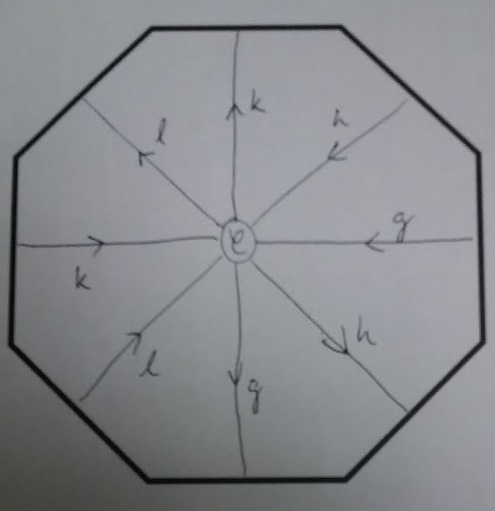
\includegraphics[width=0.5\textwidth]{basis.jpg}
\caption{Element of the spanning set $S$ for a genus 2 surface}
\label{fig:span}
\end{figure}

\begin{figure}
 \centering
 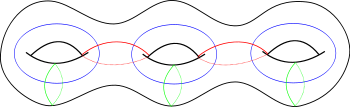
\includegraphics[width=.60\textwidth]{lickorish.png}
 \caption{Simple closed curves for the Dehn twists in the Lickorish generating set for the mapping class group of a genus $3$ closed surface (Image source: \url{https://en.wikipedia.org/wiki/Dehn_twist})}
\label{fig:lickorish}
\end{figure}



The mapping class group of $\Si$ is generated by the Lickorish generating set consisting of Dehn twists around $3g-1$ simple closed curves.   These can be divided into two types of twists: the ones around a single hole (the blue and green curves in Figure \ref{fig:lickorish}), and the ones connecting two holes (the red curves). The action of a Dehn twist around a simple closed curve corresponds to cutting the manifold along the curve, holding one piece in place and twisting the other piece by $2\pi$ radians in a clockwise direction, then gluing the two pieces back together.


To understand the action of each type of Dehn twist on the representation space $H$, we will consider the action on the spanning set $S$.  First, we claim that we can apply local moves to any element of $S$ to get a colored graph of the form shown in the first subfigure of Figure \ref{fig:tikzTwist1_1}, where the unshown part of the fundamental polygon looks the same as in the definition of $S$.  Indeed, to pass from an arbitrary element of $S$, to a colored graph of the form shown in the first subfigure of $\ref{fig:tikzTwist1_1}$, we first add coevalution-labeled vertices to each  edge intersecting the three shown sides of the fundamental polygon.  Then connect the new vertices using edges labeled by the trivial object (this corresponds to applying the second local move in Figure \ref{f:local_rels1} with  $k = 0$), contract the connections to get one new vertex, and tensor together the edges connecting the old vertex to the new vertex.

The action of the first type of Dehn twist on an arbitrary element of $S$ is shown in the first two subfigures of Figure \ref{fig:tikzTwist1_1}.  
After applying the Dehn twist, we have the simple colored graph shown in the second subfigure of Figure \ref{fig:tikzTwist1_1}.  We then apply local moves in the remaining subfigures.  For example, to go from the second subfigure to the third, we first apply the third local move of Figure \ref{f:local_rels1} to add a $\coev$-labeled vertex to the top left $g$-labeled edge.  We then apply the second local move (tensoring edges) with the number of parallel edges $k = 0$ to add an edge labeled by the trivial object between the new vertex and the old one. To go from the third to the fourth subfigure, we apply the edge contraction local move on the new edge.  Lastly, we get to the fifth subfigure by applying the tensoring edges local move again (strictly speaking, this is not a valid move since it does not take place on a disk, but one can easily add a $\coev$-labeled vertex to each of the two parallel edges, connect them, contract the connection, tensor together each of the two pairs of parallel edges, and contract one of the resulting edges to get the same result). By repeated application of Proposition $\ref{prop:omega}$, the resulting colored graph is equivalent to $\beta \Delta$, for some $\beta \in \mu_{|G|}$ and  $\Delta \in S$.    Thus, the first type of Dehn twist maps $S$ to $\mu_{|G|} S$.

An analogous proof works for the second type of Dehn twist shown in Figure \ref{fig:tikzTwist2_0}. Thus, the image of any such mapping class group representation is a quotient of the group of permutations of the finite set $\mu_{|G|} S$, hence finite.
\end{proof}

\begin{rmk} 
When $\omega = 1$ and $\Si$ is closed, this representation is a permutation representation.  
\end{rmk}

\begin{proof}
Under the assumption that the representation in \cite{fjfu} coincides with ours, this fact follows from Theorem 2.6 in \cite{fjfu}, but we can also prove it directly.  We first note that $G$ acts on $S$ by simultaneous conjugation of all edge labels by a single element $g \in G$.  If $s \in S$ and $g \in G$, then we can retrieve $s$ from $gs$ by separating two oppositely oriented, $g$-labeled edges from each edge in the embedded graph $gs$.  This results in a loop labeled by $g$, whose evaluation is $1$.  Thus $gs$ is equivalent to $s$.  Moreover, the cardinality $|S/G| = |\Hom(\pi_1(M), G)|/|G|$ is equal to the dimension of the untwisted Dijkgraaf-Witten representation space $H$ \cite{dijkgraaf1990}.  Hence, $S/G$ is a basis for $H$.  The mapping class group action on $S$ commutes with the $G$-action, so the mapping class group permutes $S/G$, i.e. $H$ is a permutation representation.
\end{proof}

\newcommand{\nc}{\newcommand}
\newcommand{\rnc}{\renewcommand}

%% Definitions

    % boundary of polygon
    % top left corner
     \nc{\lcx}{-0.5}
     \nc{\lcy}{0.866}
     \nc{\rcx}{-\lcx}
     \nc{\rcy}{\lcy}

     %TODO: Color edges
     \nc{\makeBdy}{
       \begin{scope}[very thick,decoration={
             markings,
             mark=at position 0.5 with {\arrow{>}}}
         ]  

         \draw (-1,0) -- (\lcx, \lcy); 
         \draw (\lcx, \lcy) -- (\rcx, \rcy); 
         \draw  (1, 0) -- (\rcx, \rcy);
       \end{scope}
     }

    %cut    
    % left endpoint of cut
    \nc{\lcutx}{-0.6}
    \nc{\lcuty}{0.6928}
    \nc{\lcut}{(\lcutx, \lcuty)}
    \nc{\rcutx}{-\lcutx}
    \nc{\rcuty}{\lcuty}
    \nc{\rcut}{(\rcutx, \rcuty)}

    %Main vertex
    \nc{\mvx}{0}
    \nc{\mvy}{0.2}
    \nc{\mv}{(\mvx, \mvy)}

    % outgoing edge
    \nc{\outEdge}{\draw[postaction={decorate}]  (0, 0) -- \mv node[pos=.5, right]{$hgh^{-1}$};}

    % middle of top edge of polygon
    \nc{\mtopx}{0}
    \nc{\mtopy}{0.866}
    \nc{\mtop}{(\mtopx, \mtopy)}

\begin{figure}
\centering

\begin{tabular}{|c|c|}

\hline

%Dehn twist 1.1
    \begin{tikzpicture}[scale=3]    

      % boundary of polygon
      \makeBdy


    \begin{scope}[very thick,decoration={
    markings,
    mark=at position 0.5 with {\arrow{>}}}
    ]  

      % cut for Dehn twist
      \draw[loosely dashed] \lcut -- \rcut;
      

      %graph edges

      \draw[postaction={decorate}]   \mv -- (0.75, 0.433) node[pos=.5,sloped,above]{$h$};
      \draw[postaction={decorate}]   \mv -- \mtop node[pos=.5,left]{$g$};
      \draw[postaction={decorate}]  (-0.75, 0.433) -- \mv node[pos=.5,sloped,above]{$h$};
      \outEdge

    \end{scope}
    \end{tikzpicture}

&

%1.2
    \begin{tikzpicture}[scale=3]
    
    %boundary of polygon
      \makeBdy

    %graph edges
    \begin{scope}[very thick,decoration={
    markings,
    mark=at position 0.5 with {\arrow{>}}}
    ] 


        \draw[postaction={decorate}]   \mv -- (0.75, 0.433) node[pos=.5,sloped,above]{$h$};
        % old g
        % \draw[postaction={decorate}]   \rb -- (0, 0.866) node[pos=.5,left]{$g$};
        \draw[postaction={decorate}]  (-0.75, 0.433) -- \mv node[pos=.5,sloped,above]{$h$};
        \outEdge

        % new g
        \draw[postaction={decorate}]  \mv -- \rcut
        node[pos=.5,sloped,above]{$g$};
        \draw[postaction={decorate}]  \lcut -- \mtop
        node[pos=.5,sloped,below]{$g$};

    \end{scope}
    \end{tikzpicture}

\\ \hline

%1.3
      \begin{tikzpicture}[scale=3]
    
    %boundary of polygon
      \makeBdy

    %graph edges
    \begin{scope}[very thick,decoration={
    markings,
    mark=at position 0.5 with {\arrow{>}}}
    ] 

        \draw[postaction={decorate}]   \mv -- (0.75, 0.433) node[pos=.5,sloped,above]{$h$};
        \draw[postaction={decorate}]  (-0.75, 0.433) -- \mv node[pos=.5,sloped,above]{$h$};

        \outEdge

        \draw[postaction={decorate}]  \mv -- \rcut
        node[pos=.5,sloped,above]{$g$};
        %\draw[postaction={decorate}]  \lcut -- \mtop
        \draw[postaction={decorate}]  \lcut --  ({(\lcutx + \mtopx)/2} , {(\lcuty + \mtopy)/2})
        node[pos=.5,sloped,below]{$g$};
        \draw[postaction={decorate}]  ({(\lcutx + \mtopx)/2} , {(\lcuty + \mtopy)/2}) -- \mtop
        node[pos=.5,sloped,below]{$g$};


        \draw  \mv --  ({(\lcutx + \mtopx)/2} , {(\lcuty + \mtopy)/2});

    \end{scope}
    \end{tikzpicture}

&

%1.4
    
    \begin{tikzpicture}[scale=3]

      %boundary of polygon
      \makeBdy


      
      \begin{scope}[very thick,decoration={
            markings,
            mark=at position 0.5 with {\arrow{>}}}
        ] 
      %graph edges

        \draw[postaction={decorate}]   \mv -- (0.75, 0.433) node[pos=.5,sloped,above]{$h$};
        \draw[postaction={decorate}]  (-0.75, 0.433) -- \mv node[pos=.5,sloped,above]{$h$};

        \outEdge

        \draw[postaction={decorate}]  \mv -- \rcut
        node[pos=.5,sloped,above]{$g$};
        %\draw[postaction={decorate}]  \lcut -- \mtop
        \draw[postaction={decorate}]  \lcut -- \mv
        node[pos=.5,sloped,above]{$g$};
        \draw[postaction={decorate}]  \mv -- \mtop
        node[pos=.5,right]{$g$};


    \end{scope}
    \end{tikzpicture}

\\ \hline

%Dehn twist 1.5

    
    \begin{tikzpicture}[scale=3]

    % boundary of polygon
     \makeBdy
    
    %graph edges
    \begin{scope}[very thick,decoration={
    markings,
    mark=at position 0.5 with {\arrow{>}}}
    ]  
        \draw[postaction={decorate}]   \mv -- (0.75, 0.433) node[pos=.5,sloped,above]{$hg$};
        \draw[postaction={decorate}]   \mv -- \mtop node[pos=.5,left]{$g$};
        \draw[postaction={decorate}]  (-0.75, 0.433) -- \mv node[pos=.5,sloped,above]{$hg$};
        \outEdge

    \end{scope}
    \end{tikzpicture}

&

\\ \hline
\end{tabular}

\caption{Using local moves to calculate the action of the first type of Dehn twist on an arbitrary element of the spanning set $S$. Read from left to right, then top to bottom.  Unlabeled interior edges are colored by the group identity element.  The Dehn twist is performed along the dashed simple closed curve.  The first two subfigures show the action of the Dehn twist.  The last three show the local moves relating the image of the Dehn twist to another element of $S$.}
\label{fig:tikzTwist1_1}
\end{figure}

%%%%%%%%%%%% Twist 2 %%%%%%%%%%%%%%%%


\nc{\makeBdyTwo}{
  \begin{scope}[very thick,decoration={
    markings,
    mark=at position 0.5 with {\arrow{>}}}
    ]  
    \path[draw]
    (1.0,          0.0) --       %0
    (0.92388,      0.382683)  -- %1
    (0.707107,     0.707107) --  %2
    (0.382683,     0.92388) --   %3
    (0,            1.0)   --     %4
    (-0.382683,    0.92388) --   %5
    (-0.707107 ,   0.707107)  -- %6
    ( -0.92388,    0.382683) --  %7
    ( -1.0     ,   0);           %8

  \end{scope}
}


\nc{\mvTwo}{ (-0.312076, 0.753418) }

\nc{\outEdgeTwo}{\draw[postaction={decorate}]  (0, 0) -- \mv node[pos=.3, right]{$[a,b][c,d]$};}

% 0.9 1 + 0.1 6
\nc{\cutOneX}{{0.8*(-0.92388) + 0.2*(-0.707107)}}
\nc{\cutOneY}{{0.8*(0.382683) + 0.2*(0.707107)}}
\nc{\cutOne}{(\cutOneX, \cutOneY)}

%0.9 3 + 0.1 4
\nc{\cutTwoX}{{0.8*(0.382683) + 0.2*(0)}}
\nc{\cutTwoY}{{0.8*(0.92388) + 0.2*(1.0)}}
\nc{\cutTwo}{(\cutTwoX, \cutTwoY)}

%0.9 2 + 0.1 1
\nc{\cutThreeX}{{0.8*(0.707107 ) + 0.2*(0.92388 )}}
\nc{\cutThreeY}{{0.8*(0.707107 ) + 0.2*(0.382638 )}}
\nc{\cutThree}{(\cutThreeX, \cutThreeY)}

%0.9 2 + 0.1 3
\nc{\cutFourX}{{0.2*( 0.382683) + 0.8*(0.707107)}}
\nc{\cutFourY}{{0.2*( 0.92388) + 0.8*(0.707107)}}
\nc{\cutFour}{(\cutFourX, \cutFourY)}

%0.1 0   0.9 1
\nc{\cutFiveX}{{0.2*( 1.0) + 0.8*(0.92388)}}
\nc{\cutFiveY}{{0.2*( 0.0) + 0.8*(0.382638)}}
\nc{\cutFive}{(\cutFiveX, \cutFiveY)}

%0.1 2   0.9 1
\nc{\cutSixX}{{0.2*( 0.707107) + 0.8*(0.92388)}}
\nc{\cutSixY}{{0.2*( 0.707107) + 0.8*(0.382683)}}
\nc{\cutSix}{(\cutSixX, \cutSixY)}

%0.1 3      0.9 4
\nc{\cutSevenX}{{0.2*( 0.382683) + 0.8*(0.0)}}
\nc{\cutSevenY}{{0.2*( 0.92388) + 0.8*(1.0)}}
\nc{\cutSeven}{(\cutSevenX, \cutSevenY)}

%0.1 5 0.9 4
\nc{\cutEightX}{{0.2*( -0.382683) + 0.8*(0.0)}}
\nc{\cutEightY}{{0.2*( 0.92388) + 0.8*(1.0)}}
\nc{\cutEight}{(\cutEightX, \cutEightY)}

\begin{figure}
\centering

\begin{tabular}{|c|c|}

\hline
%2.1    
    \begin{tikzpicture}[scale=3]

    % boundary of polygon
     \makeBdyTwo

     % cut for Dehn twist
     \draw[dotted] \cutOne -- \cutTwo;
     \draw[dotted] \cutThree -- \cutFour;
     \draw[dotted] \cutFive -- \cutSix;
     \draw[dotted] \cutSeven -- \cutEight;
         
    %graph edges
    \begin{scope}[very thick,decoration={
    markings,
    mark=at position 0.5 with {\arrow{>}}}
    ]  
       \draw[postaction={decorate}]  \mv -- (   0.96194 , 0.191342) node[pos=.5,sloped,above]{$a$};
       \draw[postaction={decorate}]  \mv -- ( 0.815493,  0.544895) node[pos=.5,sloped,above]{$b$};
       \draw[postaction={decorate}] (0.544895,  0.815493) -- \mv  node[pos=.5,sloped,above]{$a$};
       \draw[postaction={decorate}]   (0.191342,  0.96194) -- \mv  node[pos=.4,sloped,above]{$b$}; 
       \draw[postaction={decorate}]  \mv -- (-0.191342,  0.96194) node[pos=.4,sloped,above]{$c$}; 
       \draw[postaction={decorate}]  \mv -- (-0.544895,  0.815493) node[pos=.5,sloped,above]{$d$}; 
       \draw[postaction={decorate}] (-0.815493,  0.544895) -- \mv  node[pos=.5,sloped,above]{$c$};
       \draw[postaction={decorate}] (-0.96194,   0.191342) -- \mv  node[pos=.5,sloped,above]{$d$};

         \outEdgeTwo
    \end{scope}
    \end{tikzpicture}

&

%2.2
    
    \begin{tikzpicture}[scale=3]

    % boundary of polygon
     \makeBdyTwo

     % cut for Dehn twist
     \draw[dotted] \cutOne -- \cutTwo;
     \draw[dotted] \cutThree -- \cutFour;
     \draw[dotted] \cutFive -- \cutSix;
     \draw[dotted] \cutSeven -- \cutEight;
         
    %graph edges
    \begin{scope}[very thick,decoration={
    markings,
    mark=at position 0.5 with {\arrow{>}}}
    ]  
       \draw[postaction={decorate}]  \mv -- \mvTwo node[pos=.5,sloped,above]{\tiny $g := b^{-1}cdc^{-1}$};

       \draw[postaction={decorate}]  \mv -- (   0.96194 , 0.191342) node[pos=.5,sloped,above]{$a$};
       \draw[postaction={decorate}]  \mv -- ( 0.815493,  0.544895) node[pos=.5,sloped,above]{$b$};
       \draw[postaction={decorate}] (0.544895,  0.815493) -- \mv  node[pos=.5,sloped,above]{$a$};
       \draw[postaction={decorate}]   (0.191342,  0.96194) -- \mvTwo  node[pos=.5,sloped,above]{$b$}; 
       \draw[postaction={decorate}]  \mvTwo -- (-0.191342,  0.96194) node[pos=.5,sloped,above]{$c$}; 
       \draw[postaction={decorate}]  \mvTwo -- (-0.544895,  0.815493) node[pos=.5,sloped,above]{$d$}; 
       \draw[postaction={decorate}] (-0.815493,  0.544895) -- \mvTwo  node[pos=.5,sloped,above]{$c$};
       \draw[postaction={decorate}] (-0.96194,   0.191342) -- \mv  node[pos=.5,sloped,above]{$d$};

         \outEdgeTwo
    \end{scope}
    \end{tikzpicture}

\\ \hline

%2.3
    
    \begin{tikzpicture}[scale=3]

    % boundary of polygon
     \makeBdyTwo
         
    %graph edges
    \begin{scope}[very thick,decoration={
    markings,
    mark=at position 0.5 with {\arrow{>}}}
    ]  
       \draw[postaction={decorate}]  \mv -- \cutTwo node[pos=.5,sloped,above]{$g$};
       \draw[postaction={decorate}]  \cutOne -- \mvTwo node[pos=.5,sloped,below]{$g$};
       \draw[postaction={decorate}]  \cutThree -- \cutFour node[pos=.5,sloped,below]{$g$};
       \draw[postaction={decorate}]  \cutFive -- \cutSix node[pos=.5,sloped,below]{$g$};
       \draw[postaction={decorate}]  \cutSeven -- \cutEight node[pos=.5,sloped,red]{$g$};


       \draw[postaction={decorate}]  \mv -- (   0.96194 , 0.191342) node[pos=.5,sloped,above]{$a$};
       \draw[postaction={decorate}]  \mv -- ( 0.815493,  0.544895) node[pos=.5,sloped,above]{$b$};
       \draw[postaction={decorate}] (0.544895,  0.815493) -- \mv  node[pos=.5,sloped,above]{$a$};
       \draw[postaction={decorate}]   (0.191342,  0.96194) -- \mvTwo  node[pos=.5,sloped,below]{$b$}; 
       \draw[postaction={decorate}]  \mvTwo -- (-0.191342,  0.96194) node[pos=.5,sloped,above]{$c$}; 
       \draw[postaction={decorate}]  \mvTwo -- (-0.544895,  0.815493) node[pos=.5,sloped,above]{$d$}; 
       \draw[postaction={decorate}] (-0.815493,  0.544895) -- \mvTwo  node[pos=.5,sloped,above]{$c$};
       \draw[postaction={decorate}] (-0.96194,   0.191342) -- \mv  node[pos=.5,sloped,above]{$d$};

         \outEdgeTwo
    \end{scope}
    \end{tikzpicture}

&

%2.4
    
    \begin{tikzpicture}[scale=3]

    % boundary of polygon
     \makeBdyTwo
         
    %graph edges
    \begin{scope}[very thick,decoration={
    markings,
    mark=at position 0.5 with {\arrow{>}}}
    ]  
       \draw[postaction={decorate}]  \mv -- \cutTwo node[pos=.5,sloped,above]{$g$};
       \draw[postaction={decorate}]  \cutThree -- \mv node[pos=.3,sloped,above]{$g$};

       \draw[postaction={decorate}]  \mv -- ( 0.96194 , 0.191342) node[pos=.8,sloped,above]{$ag^{-1}$};
       \draw[postaction={decorate}]  \mv -- ( 0.815493,  0.544895) node[pos=.7,sloped,below]{$gb$};
       \draw[postaction={decorate}] (0.544895,  0.815493) -- \mv  node[pos=.2,sloped,above]{$ag^{-1}$};
       \draw[postaction={decorate}]   (0.191342,  0.96194) -- \mvTwo  node[pos=.5,sloped,below]{$gb$}; 
       \draw[postaction={decorate}]  \mvTwo -- (-0.191342,  0.96194) node[pos=.5,sloped,above]{$gc$}; 
       \draw[postaction={decorate}]  \mvTwo -- (-0.544895,  0.815493) node[pos=.5,sloped,above]{$d$}; 
       \draw[postaction={decorate}] (-0.815493,  0.544895) -- \mvTwo  node[pos=.5,sloped,below]{$gc$};
       \draw[postaction={decorate}] (-0.96194,   0.191342) -- \mv  node[pos=.5,sloped,above]{$d$};

         \outEdgeTwo
    \end{scope}
    \end{tikzpicture}

\\ \hline 

%2.5

    \begin{tikzpicture}[scale=3]

    % boundary of polygon
     \makeBdyTwo
         
    %graph edges
    \begin{scope}[very thick,decoration={
    markings,
    mark=at position 0.5 with {\arrow{>}}}
    ]  
       \draw[postaction={decorate}]  \mv -- \cutTwo node[pos=.8,sloped,red]{$g$};
       \draw[postaction={decorate}]  \cutThree -- \mv node[pos=.2,sloped,above]{$g$};

       \draw[postaction={decorate}]  \mv -- ( 0.96194 , 0.191342) node[pos=.8,sloped,above]{$ag^{-1}$};
       \draw[postaction={decorate}]  \mv -- ( 0.815493,  0.544895) node[pos=.7,sloped,below]{$gb$};
       \draw[postaction={decorate}] (0.544895,  0.815493) -- \mv  node[pos=.2,sloped,above]{$ag^{-1}$};
       \draw[postaction={decorate}]   (0.191342,  0.96194) -- \mv  node[pos=.2,sloped,above]{$gb$}; 
       \draw[postaction={decorate}]  \mv -- (-0.191342,  0.96194) node[pos=.8,sloped,below]{$gc$}; 
       \draw[postaction={decorate}]  \mv -- (-0.544895,  0.815493) node[pos=.7,sloped,above]{$d$}; 
       \draw[postaction={decorate}] (-0.815493,  0.544895) -- \mv  node[pos=.3,sloped,above]{$gc$};
       \draw[postaction={decorate}] (-0.96194,   0.191342) -- \mv  node[pos=.3,sloped,above]{$d$};

         \outEdgeTwo
    \end{scope}
    \end{tikzpicture}

&

%2.6

    \begin{tikzpicture}[scale=3]

    % boundary of polygon
     \makeBdyTwo
         
    %graph edges
    \begin{scope}[very thick,decoration={
    markings,
    mark=at position 0.5 with {\arrow{>}}}
    ]  

       \draw[postaction={decorate}]  \mv -- ( 0.96194 , 0.191342) node[pos=.8,sloped,above]{$ag^{-1}$};
       \draw[postaction={decorate}]  \mv -- ( 0.815493,  0.544895) node[pos=.8,sloped,above]{$gbg^{-1}$};
       \draw[postaction={decorate}] (0.544895,  0.815493) -- \mv  node[pos=.2,sloped,above]{$ag^{-1}$};
       \draw[postaction={decorate}]   (0.191342,  0.96194) -- \mv  node[pos=.2,sloped,above]{$gbg^{-1}$}; 
       \draw[postaction={decorate}]  \mv -- (-0.191342,  0.96194) node[pos=.8,sloped,below]{$gc$}; 
       \draw[postaction={decorate}]  \mv -- (-0.544895,  0.815493) node[pos=.7,sloped,above]{$d$}; 
       \draw[postaction={decorate}] (-0.815493,  0.544895) -- \mv  node[pos=.3,sloped,above]{$gc$};
       \draw[postaction={decorate}] (-0.96194,   0.191342) -- \mv  node[pos=.3,sloped,above]{$d$};

         \outEdgeTwo
    \end{scope}
    \end{tikzpicture}

\\ \hline
\end{tabular}

\caption{Using local moves to calculate the action of the second type of Dehn twist on an arbitrary element of the spanning set $S$. Read from left to right, then top to bottom.   The Dehn twist is performed along the dashed simple closed curve.  The first two subfigures show application of local moves prior to the Dehn twist action. The third shows the action of the twist.  The last three show the local moves relating the image of the Dehn twist to another element of $S$.}
\label{fig:tikzTwist2_0}
\end{figure}


\subsection{Boundary Case}

When $\Si$ has boundary, we denote by $\MCG(\Si)$ the group of isotopy classes of homeomorphisms fixing the boundary of $\Si$ setwise. Given any labelling of the boundary  by objects in the Drinfeld center, $l : \pi_0(\partial M) \to \Obj(Z(\vgo))$, we get a mapping class group representation. The representation space is $\Hs(\Si, \VV)$ with boundary condition $\VV = F \circ l$, where $F$ is the forgetful functor $F: Z(\vgo) \to \vgo$.  The same local relations are valid in this representation space \cite{kirillovStringNets}.

By a similar argument as in the proof of the Theorem $\ref{thm:closed}$, any such representation space has a finite spanning set $S$ consisting of all simple colored graphs with a single vertex, loops for each of the usual generators of the fundamental group of $\Si$, and a leg from the vertex to each of the boundary components.  

Let $N$ denote the closed surface obtained by filling in all the boundary components of $\Si$ with disks. The mapping class group $\MCG(\Si)$ is generated by the same Dehn twists as $\MCG(N)$, as well as braids interchanging boundary components and mapping classes corresponding to dragging a boundary component along a representative of a standard generator of $\pi_1(N)$ \cite{birman}.  As in the proof of Theorem \ref{thm:closed}, applying any of these generators of $\MCG(\Si)$ to a colored graph in $S$ yields an element in $\mu_{|G|}S$ (see Figures \ref{fig:braid1} and \ref{fig:drag1}).  Since the braid group is also generated by such braids, we have the following theorem.


\nc{\rightX}{0.5}  % left marked point x value
\nc{\leftX}{-\rightX} % right marked point x value
\nc{\pY}{0.5}  % y value for marked points
\nc{\loopR}{0.3}
\renewcommand{\mv}{(0, -0.2)}

\nc{\makeBase}{
      % left loop
       \draw[very thick]  \mv -- ({\leftX - \loopR}, \pY);
       \draw[very thick]   ({\leftX + \loopR}, \pY) -- \mv;
       
       \begin{scope}[very thick,decoration={
             markings,
             mark=at position 0.5 with {\arrow{>}}}
         ]  

         % left leg
         \draw[postaction={decorate}]  \mv -- (\leftX, \pY) node[pos=.5,above]{$l$};

       \end{scope}

       % new right loop and leg
       \draw[very thick]  \mv -- ({\leftX - 4*\loopR}, \pY);
       \draw[very thick]   ({\leftX - 2*\loopR}, \pY) -- \mv;
 
       % right leg
       \draw[very thick]  \mv -- ({\leftX - 3*\loopR}, \pY);       

}


\nc{\makeBaseTwo}{
    % left loop

       \draw[very thick]   ({\leftX + \loopR}, \pY) -- \mv;
       
       \begin{scope}[very thick,decoration={
             markings,
             mark=at position 0.5 with {\arrow{>}}}
         ]  

         % left leg
         \draw[postaction={decorate}]  \mv -- (\leftX, \pY) node[pos=.5,above]{$l$};

       \end{scope}
  
       \draw[very thick]   ({\leftX - 2*\loopR}, \pY) -- \mv;
}


%bottom right of right loop
\nc{\bRight}{
        \begin{scope}[very thick,decoration={
           markings,
           mark=at position 0.5 with {\arrow{>}}}
       ]  
       \draw[postaction={decorate}]   plot[domain=360:180] ({\loopR*cos(\x) + \leftX + 3*\loopR}, {\loopR*sin(\x) + \pY});
       \node[below] at  ({\loopR*cos(270) + \leftX + 3*\loopR}, {\loopR*sin(270) + \pY}) {$g$};
     \end{scope}
   }

\nc{\makeBraid}{

     \makeBase

     \begin{scope}[very thick,decoration={
           markings,
           mark=at position 0.5 with {\arrow{>}}}
       ]  

       % left loop
       \draw[postaction={decorate}]   plot[domain=180:0]  
              ({\loopR*cos(\x) + \leftX}, {\loopR*sin(\x) + \pY});
       \node[above] at  ({\loopR*cos(90) + \leftX}, {\loopR*sin(90) + \pY}) {$k$};

       % right loop
       \draw[postaction={decorate}]     plot[domain=0:180] ({2*\loopR*cos(\x) + \leftX}, {2*\loopR*sin(\x) + \pY});
       \node[above] at  ({2*\loopR*cos(90) + \leftX}, {2*\loopR*sin(90) + \pY}) {$g$};
       \draw[postaction={decorate}]      plot[domain=180:0] ({4*\loopR*cos(\x) + \leftX}, {4*\loopR*sin(\x) + \pY});
       \node[above] at  ({4*\loopR*cos(90) + \leftX}, {4*\loopR*sin(90) + \pY}) {$g$};

       %\right leg
       \draw[postaction={decorate}]      plot[domain=180:0] ({3*\loopR*cos(\x) + \leftX}, {3*\loopR*sin(\x) + \pY});
       \node[above] at  ({3*\loopR*cos(90) + \leftX}, {3*\loopR*sin(90) + \pY}) {$h$};

     \end{scope}

     \bRight
       
}


\nc{\makeBraidOne}{

     \makeBase

     \begin{scope}[very thick,decoration={
           markings,
           mark=at position 0.25 with {\arrow{>}},
          mark=at position 0.75 with {\arrow{>}}}
       ]  

       % left loop
       \draw[postaction={decorate}]   plot[domain=180:0]  
              ({\loopR*cos(\x) + \leftX}, {\loopR*sin(\x) + \pY});
       \node[above] at  ({\loopR*cos(45) + \leftX}, {\loopR*sin(45) + \pY}) {$k$};
       \node[above] at  ({\loopR*cos(135) + \leftX}, {\loopR*sin(135) + \pY}) {$k$};

       % right loop
       \draw[postaction={decorate}]     plot[domain=0:180] ({2*\loopR*cos(\x) + \leftX}, {2*\loopR*sin(\x) + \pY});
       \node[above] at  ({2*\loopR*cos(45) + \leftX}, {2*\loopR*sin(45) + \pY}) {$g$};
       \node[above] at  ({2*\loopR*cos(135) + \leftX}, {2*\loopR*sin(135) + \pY}) {$g$};
       \draw[postaction={decorate}]      plot[domain=180:0] ({4*\loopR*cos(\x) + \leftX}, {4*\loopR*sin(\x) + \pY});
       \node[above] at  ({4*\loopR*cos(45) + \leftX}, {4*\loopR*sin(45) + \pY}) {$g$};
       \node[above] at  ({4*\loopR*cos(135) + \leftX}, {4*\loopR*sin(135) + \pY}) {$g$};

       %\right leg
       \draw[postaction={decorate}]      plot[domain=180:0] ({3*\loopR*cos(\x) + \leftX}, {3*\loopR*sin(\x) + \pY});
       \node[above] at  ({3*\loopR*cos(45) + \leftX}, {3*\loopR*sin(45) + \pY}) {$h$};
       \node[above] at  ({3*\loopR*cos(135) + \leftX}, {3*\loopR*sin(135) + \pY}) {$h$};

     \end{scope}

     \bRight       
}


\nc{\makeBraidTwo}{

     \makeBase


     \begin{scope}[very thick,decoration={
           markings,
           mark=at position 0.1 with {\arrow{>}},
          mark=at position 0.9 with {\arrow{>}}}
       ]  
       % \right leg
       \draw[postaction={decorate}]      plot[domain=180:0] ({3*\loopR*cos(\x) + \leftX}, {3*\loopR*sin(\x) + \pY});
       \node[right] at  ({3*\loopR*cos(18) + \leftX}, {3*\loopR*sin(18) + \pY}) {$h$};
       \node[left] at  ({3*\loopR*cos(162) + \leftX}, {3*\loopR*sin(162) + \pY}) {$h$};

       % left loop
       \draw[postaction={decorate}]      plot[domain=180:0] ({\loopR*cos(\x) + \leftX}, {3*\loopR*sin(\x) + \pY});
       \node[left] at  ({\loopR*cos(18) + \leftX}, {3*\loopR*sin(18) + \pY}) {$k$};
       \node[left] at  ({\loopR*cos(162) + \leftX}, {3*\loopR*sin(162) + \pY}) {$k$};
     \end{scope}

       % right loop
     \begin{scope}[very thick,decoration={
           markings,
           mark=at position 0.9 with {\arrow{>}}}]
       \draw[postaction={decorate}]         plot[domain=0:180] ({2*\loopR*cos(\x) + \leftX}, {3*\loopR*sin(\x) + \pY});
       \node[left] at  ({2*\loopR*cos(162) + \leftX}, {3*\loopR*sin(162) + \pY}) {$g$};
     \end{scope}
     \begin{scope}[very thick,decoration={
           markings,
           mark=at position 0.1 with {\arrow{>}}}]
     \draw[postaction={decorate}]       plot[domain=180:0] ({4*\loopR*cos(\x) + \leftX}, {3*\loopR*sin(\x) + \pY});
       \node[left] at  ({4*\loopR*cos(162) + \leftX}, {3*\loopR*sin(162) + \pY}) {$g$};
     \end{scope}
         
       \bRight
}

\nc{\makeBraidThree}{

  \makeBaseTwo

     \begin{scope}[very thick,decoration={
           markings,
          mark=at position 0.8 with {\arrow{>}}}
       ]  
       % \right leg
       \draw[postaction={decorate}]      plot[domain=90:0] ({3*\loopR*cos(\x) + \leftX}, {3*\loopR*sin(\x) + \pY});
       \node[right] at  ({3*\loopR*cos(18) + \leftX}, {3*\loopR*sin(18) + \pY}) {$h$};

       % left loop
       \draw[postaction={decorate}]      plot[domain=90:0] ({\loopR*cos(\x) + \leftX}, {3*\loopR*sin(\x) + \pY});
       \node[left] at  ({\loopR*cos(18) + \leftX}, {3*\loopR*sin(18) + \pY}) {$k$};
     \end{scope}

       % right loop
     \begin{scope}[very thick,decoration={
           markings,
           mark=at position 0.1 with {\arrow{>}}}]
       \draw[postaction={decorate}]         plot[domain=180:0] ({2*\loopR*cos(\x) + \leftX}, {3*\loopR*sin(\x) + \pY});
       \node[left] at  ({2*\loopR*cos(162) + \leftX}, {3*\loopR*sin(162) + \pY}) {$kg^{-1}hg$};
     \end{scope}

     \draw[very thick]       plot[domain=90:0] ({4*\loopR*cos(\x) + \leftX}, {3*\loopR*sin(\x) + \pY});
         
       \bRight
}


\begin{figure}
\centering

\begin{tabular}{|c|c|}

  \hline
  
  %Braid 1
    \begin{tikzpicture}[scale=2.5]

         
    %graph edges
    \begin{scope}[very thick,decoration={
    markings,
    mark=at position 0.5 with {\arrow{>}}}
    ]  


       % left loop
       \draw  \mv -- ({\leftX - \loopR}, \pY);
       \draw[postaction={decorate}]    plot[domain=180:0] ({\loopR*cos(\x) + \leftX}, {\loopR*sin(\x) + \pY});
       \node[above] at ({\loopR*cos(90) + \leftX}, {\loopR*sin(90) + \pY}) {$g$};
       \draw   ({\leftX + \loopR}, \pY) -- \mv;
       
       % left leg
       \draw[postaction={decorate}]  \mv -- (\leftX, \pY) node[pos=.5,above]{$h$};

       % right loop
       \draw  \mv -- ({\rightX - \loopR}, \pY);
       \draw[postaction={decorate}] plot[domain=180:0] ({\loopR*cos(\x) + \rightX}, {\loopR*sin(\x) + \pY});
       \node[above] at ({\loopR*cos(90) + \rightX}, {\loopR*sin(90) + \pY}) {$k$};
       \draw   ({\rightX + \loopR}, \pY) -- \mv;
 
       % right leg
       \draw[postaction={decorate}]  \mv -- (\rightX, \pY) node[pos=.5, above]{$l$};       
  
    \end{scope}
    \end{tikzpicture}

&

  %Braid 2
    \begin{tikzpicture}[scale=2.5]

         
    %graph edges
    \begin{scope}[very thick,decoration={
    markings,
    mark=at position 0.5 with {\arrow{>}}}
    ]  

    \makeBraid
  
    \end{scope}
    \end{tikzpicture}

\\ \hline

  %Braid 3
    \begin{tikzpicture}[scale=2.5]

      \makeBraidOne
         
    %graph edges
    \begin{scope}[very thick,decoration={
    markings,
    mark=at position 0.5 with {\arrow{>}}}
    ]  

       % connecting edge
       \draw ({\leftX}, {\pY + \loopR}) -- ({\leftX}, {\pY + 4*\loopR});
  
    \end{scope}
    \end{tikzpicture}

&

  %Braid 4
    \begin{tikzpicture}[scale=2.5]

      \makeBraidTwo     
         
    \end{tikzpicture}

\\ \hline

    %Braid 5
    \begin{tikzpicture}[scale=2.5]

      \makeBraidThree
         
    \end{tikzpicture}

&

  %Braid 6
    \begin{tikzpicture}[scale=2.5]

         
    %graph edges
    \begin{scope}[very thick,decoration={
    markings,
    mark=at position 0.5 with {\arrow{>}}}
    ]  


       % left loop
       \draw  \mv -- ({\leftX - \loopR}, \pY);
       \draw[postaction={decorate}]    plot[domain=180:0] ({\loopR*cos(\x) + \leftX}, {\loopR*sin(\x) + \pY});
       \node[above] at ({\loopR*cos(90) + \leftX}, {\loopR*sin(90) + \pY}) {$kg^{-1}hg$};
       \draw   ({\leftX + \loopR}, \pY) -- \mv;
       
       % left leg
       \draw[postaction={decorate}]  \mv -- (\leftX, \pY) node[pos=.5,above]{$l$};

       % right loop
       \draw  \mv -- ({\rightX - \loopR}, \pY);
       \draw[postaction={decorate}] plot[domain=180:0] ({\loopR*cos(\x) + \rightX}, {\loopR*sin(\x) + \pY});
       \node[above] at ({\loopR*cos(90) + \rightX}, {\loopR*sin(90) + \pY}) {$g$};
       \draw   ({\rightX + \loopR}, \pY) -- \mv;
 
       % right leg
       \draw[postaction={decorate}]  \mv -- (\rightX, \pY) node[pos=.5, above]{$h$};       
  
    \end{scope}
    \end{tikzpicture}

\\ \hline
\end{tabular}

\caption{Using local moves to calculate the action of a braid generator on an arbitrary element of the spanning set $S$. Read from left to right, then top to bottom.   Unlabeled interior edges are colored by the group identity element. The first two subfigures show application of the braid generator, which interchanges the univalent vertices. The last four show the local moves relating the image to another element of $S$.}
\label{fig:braid1}
\end{figure}


%%%%%%%%%%%%%%%%%% Dragging along \pi_1 generator %%%%%%%%%

\rnc{\mv}{(0,0)}
\nc{\uv}{(0, 0.7)}
\nc{\rvx}{0.3}
\nc{\rvy}{\lcuty}
\nc{\rv}{(\rvx, \rvy)}
\nc{\lv}{(-\rvx, \lcuty)}

\nc{\cutRatio}{0.5}
\rnc{\lcutx}{{\cutRatio*(-0.5) + (1-\cutRatio)*(-1)}}
\rnc{\lcuty}{{\cutRatio*(0.866)}}
\rnc{\lcut}{(\lcutx, \lcuty)}
\rnc{\rcutx}{{\cutRatio*(0.5) + (1-\cutRatio)*(1)}}
\rnc{\rcut}{(\rcutx, \lcuty)}
\nc{\boundaryComponentx}{0}
\nc{\boundaryComponenty}{\lcuty}
\nc{\boundaryComponent}{(\boundaryComponentx, \boundaryComponenty)}

\nc{\connectorEnd}{({0.5*(-0.85)}, {0.5*0.2598 + 0.5*0.433})}

\nc{\edgeRatio}{0.9}
\nc{\lex}{{\edgeRatio*(-1) + (1-\edgeRatio)*(\lcx)}}
\nc{\ley}{{(1-\edgeRatio)*(\lcy)}}
\nc{\lev}{(\lex, \ley)}
%\nc{\rex}{{(-1)*(\lex)}}
\nc{\rex}{{\edgeRatio*(1) + (1-\edgeRatio)*(\rcx)}}
\nc{\rev}{(\rex, \ley)}

\nc{\eOneRatio}{0.8}
\nc{\leOnex}{{\eOneRatio*(-1) + (1-\eOneRatio)*(\lcx)}}
\nc{\leOney}{{(1-\eOneRatio)*(\lcy)}}
\nc{\leOnev}{(\leOnex, \leOney)}
\nc{\reOnex}{{\eOneRatio*(1) + (1-\eOneRatio)*(\rcx)}}
\nc{\reOnev}{(\reOnex, \leOney)}

\nc{\eTwoRatio}{0.7}
\nc{\leTwox}{{\eTwoRatio*(-1) + (1-\eTwoRatio)*(\lcx)}}
\nc{\leTwoy}{{(1-\eTwoRatio)*(\lcy)}}
\nc{\leTwov}{(\leTwox, \leTwoy)}
\nc{\reTwox}{{\eTwoRatio*(1) + (1-\eTwoRatio)*(\rcx)}}
\nc{\reTwov}{(\reTwox, \leTwoy)}

\nc{\eThreeRatio}{0.6}
\nc{\leThreex}{{\eThreeRatio*(-1) + (1-\eThreeRatio)*(\lcx)}}
\nc{\leThreey}{{(1-\eThreeRatio)*(\lcy)}}
\nc{\leThreev}{(\leThreex, \leThreey)}
\nc{\reThreex}{{\eThreeRatio*(1) + (1-\eThreeRatio)*(\rcx)}}
\nc{\reThreev}{(\reThreex, \leThreey)}

\nc{\eFourRatio}{0.4}
\nc{\leFourx}{{\eFourRatio*(-1) + (1-\eFourRatio)*(\lcx)}}
\nc{\leFoury}{{(1-\eFourRatio)*(\lcy)}}
\nc{\leFourv}{(\leFourx, \leFoury)}
\nc{\reFourx}{{\eFourRatio*(1) + (1-\eFourRatio)*(\rcx)}}
\nc{\reFourv}{(\reFourx, \leFoury)}

\nc{\eFiveRatio}{0.2}
\nc{\leFivex}{{\eFiveRatio*(-1) + (1-\eFiveRatio)*(\lcx)}}
\nc{\leFivey}{{(1-\eFiveRatio)*(\lcy)}}
\nc{\leFivev}{(\leFivex, \leFivey)}
\nc{\reFivex}{{\eFiveRatio*(1) + (1-\eFiveRatio)*(\rcx)}}
\nc{\reFivev}{(\reFivex, \leFivey)}


\nc{\dby}{-0.2} %diagram bottom

\begin{figure}
\centering

\begin{tabular}{|c|c|}

  \hline
  
  % Drag 1
    \begin{tikzpicture}[scale=3]    

      % boundary of polygon
      \makeBdy


    \begin{scope}[very thick,decoration={
    markings,
    mark=at position 0.5 with {\arrow{>}}}
    ]  

      % cut for Dehn twist
      \draw[loosely dashed] \lcut -- \rcut;
      

      %graph edges
      \draw[postaction={decorate}]   (0, \dby) -- \mv node[pos=.5,right]{$p:=hglkl^{-1}h^{-1}$};
      \draw[postaction={decorate}]   \mv -- \rev node[pos=.5,sloped,above]{$h$};
      \draw[postaction={decorate}]   \mv -- \rv node[pos=.5,right]{$gl$};
      \draw[postaction={decorate}]   \mv -- \boundaryComponent node[pos=.5,left]{$k$};
      \draw[postaction={decorate}]   \lv -- \mv node[pos=.5,left]{$l$};
      \draw[postaction={decorate}]   \lev -- \mv node[pos=.5,sloped,below]{$h$};

      \draw[postaction={decorate}]   \rv -- \uv;
      \draw[postaction={decorate}]   \uv -- \mtop node[pos=.5,right]{$g$};
      \draw[postaction={decorate}]   \uv -- \lv;


    \end{scope}
    \end{tikzpicture}


&


  % Drag 2
    \begin{tikzpicture}[scale=3]    

      % boundary of polygon
      \makeBdy


    \begin{scope}[very thick,decoration={
    markings,
    mark=at position 0.5 with {\arrow{>}}}
    ]  


      %graph edges
      \draw[postaction={decorate}]   (0, \dby) -- \mv node[pos=.5,right]{$p$};
      \draw[postaction={decorate}]   \mv -- \rev node[pos=.5,sloped,below]{$h$};

      \draw[postaction={decorate}]   \mv -- \reOnev node[pos=.8,sloped,red]{$gl$};
      \draw[postaction={decorate}]   \leOnev -- \rv node[pos=.5,sloped,below]{$gl$};
      \draw[postaction={decorate}]   \rv -- \leFivev node[pos=.5,sloped,above]{$gl$};
      \draw[postaction={decorate}]   \reFivev -- \uv node[pos=.5,sloped,above]{$gl$};

      \draw[postaction={decorate}]   \mv -- \reTwov node[pos=.6,sloped,red]{$k$};
      \draw[postaction={decorate}]   \leTwov -- \boundaryComponent node[pos=.5,sloped,red]{$k$};

      \draw[postaction={decorate}]   \reThreev -- \mv node[pos=.5,sloped,above]{$l$};
      \draw[postaction={decorate}]   \lv -- \leThreev;
      \draw[postaction={decorate}]   \leFourv -- \lv node[pos=.5,sloped,above]{$l$};
      \draw[postaction={decorate}]   \uv -- \reFourv node[pos=.5,sloped,below]{$l$};

      \draw[postaction={decorate}]   \lev -- \mv node[pos=.5,sloped,below]{$h$};

      \draw[postaction={decorate}]   \uv -- \mtop node[pos=.5,right]{$g$};


    \end{scope}
    \end{tikzpicture}

\\ \hline


  % Drag 3
    \begin{tikzpicture}[scale=3]    

      % boundary of polygon
      \makeBdy

    \begin{scope}[very thick,decoration={
    markings,
    mark=at position 0.5 with {\arrow{>}}}
    ]  


      %graph edges
      \draw[postaction={decorate}]   (0, \dby) -- \mv node[pos=.5,right]{$p$};
      \draw[postaction={decorate}]   \mv -- \rev node[pos=.5,sloped,below]{$h$};

      \draw[postaction={decorate}]   \mv -- \reOnev node[pos=.8,sloped,red]{$gl$};
      \draw[postaction={decorate}]   \leOnev --  (-0.35, 0.3031) node[pos=.5,sloped,below]{$gl$};
      \draw[postaction={decorate}]   (-0.35, 0.3031) -- \rv node[pos=.5,sloped,below]{$gl$};

      \draw[postaction={decorate}]   \rv -- \leFivev node[pos=.5,sloped,above]{$gl$};
      \draw[postaction={decorate}]   \reFivev -- \uv node[pos=.5,sloped,above]{$gl$};

      \draw[postaction={decorate}]   \mv -- \reTwov node[pos=.6,sloped,red]{$k$};
      \draw[postaction={decorate}]   \leTwov -- \connectorEnd node[pos=.5,sloped,red]{$k$};
      \draw[postaction={decorate}]   \connectorEnd -- \boundaryComponent node[pos=.5,sloped,red]{$k$};


      \draw[postaction={decorate}]   \reThreev -- \mv node[pos=.5,sloped,above]{$l$};
      \draw[postaction={decorate}]   \lv -- \leThreev;
      \draw[postaction={decorate}]   \leFourv -- \lv node[pos=.5,sloped,above]{$l$};
      \draw[postaction={decorate}]   \uv -- \reFourv node[pos=.5,sloped,below]{$l$};

      \draw[postaction={decorate}]   \lev -- \mv node[pos=.5,sloped,below]{$h$};

      \draw[postaction={decorate}]   \uv -- \mtop node[pos=.5,right]{$g$};

      \draw \lcut -- \lv;
      \draw \rv -- \rcut;
      \draw \mv -- \connectorEnd;
     
    \end{scope}
    \end{tikzpicture}

&


  % Drag 4
    \begin{tikzpicture}[scale=3]    

      % boundary of polygon
      \makeBdy

    \begin{scope}[very thick,decoration={
    markings,
    mark=at position 0.5 with {\arrow{>}}}
    ]  


      %graph edges
      \draw[postaction={decorate}]   (0, \dby) -- \mv node[pos=.5,right]{$p$};
      \draw[postaction={decorate}]   \mv -- \rev node[pos=.5,sloped,below]{$h$};

      \draw[postaction={decorate}]   \mv -- \reOnev node[pos=.5,sloped,above]{$glk$};
      \draw[postaction={decorate}]   \leOnev --  (-0.35, 0.3031) node[pos=.5,sloped,above]{$glk$};
      \draw[postaction={decorate}]   (-0.35, 0.3031) -- \rv node[pos=.5,sloped,below]{$gl$};

      \draw[postaction={decorate}]   \rv -- \leFivev node[pos=.5,sloped,above]{$gl$};
      \draw[postaction={decorate}]   \reFivev -- \uv node[pos=.5,sloped,above]{$gl$};

      \draw[postaction={decorate}]    (-0.35, 0.3031)  -- \boundaryComponent node[pos=.5,sloped,above]{$k$};


      \draw[postaction={decorate}]   \rv -- \mv node[pos=.5,right]{$l$};
      \draw[postaction={decorate}]   \uv -- \rv node[pos=.5,right]{$l$};

      \draw[postaction={decorate}]   \lev -- \mv node[pos=.5,sloped,below]{$h$};

      \draw[postaction={decorate}]   \uv -- \mtop node[pos=.5,right]{$g$};


      \draw \mv --  (-0.35, 0.3031);
     
    \end{scope}
    \end{tikzpicture}


\\ \hline

  % Drag 5

 \begin{tikzpicture}[scale=3]    

      % boundary of polygon
      \makeBdy

    \begin{scope}[very thick,decoration={
    markings,
    mark=at position 0.5 with {\arrow{>}}}
    ]  


      %graph edges
      \draw[postaction={decorate}]   (0, \dby) -- \mv node[pos=.5,right]{$p$};
      \draw[postaction={decorate}]   \mv -- \rev node[pos=.5,sloped,below]{$hglk$};

      \draw[postaction={decorate}]   \rv -- \leFivev node[pos=.5,sloped,above]{$gl$};
      \draw[postaction={decorate}]   \reFivev -- \uv node[pos=.5,sloped,above]{$gl$};

      \draw[postaction={decorate}]    \mv  -- \boundaryComponent node[pos=.5,left]{$k$};


      \draw[postaction={decorate}]   \mv -- \rv node[pos=.5,right]{$l^{-1}gl$};
      \draw[postaction={decorate}]   \uv -- \rv node[pos=.5,right]{$l$};

      \draw[postaction={decorate}]   \lev -- \mv node[pos=.5,sloped,below]{$hglk$};

      \draw[postaction={decorate}]   \uv -- \mtop node[pos=.5,right]{$g$};
     
    \end{scope}
    \end{tikzpicture}

&


  % Drag 6

 \begin{tikzpicture}[scale=3]    

      % boundary of polygon
      \makeBdy

    \begin{scope}[very thick,decoration={
    markings,
    mark=at position 0.5 with {\arrow{>}}}
    ]  


      %graph edges
      \draw[postaction={decorate}]   (0, \dby) -- \mv node[pos=.5,right]{$p$};
      \draw[postaction={decorate}]   \mv -- \rev node[pos=.5,sloped,below]{$hglk$};

      \draw[postaction={decorate}]   \uv -- \leFivev node[pos=.5,sloped,below]{$gl$};
      \draw[postaction={decorate}]   \reFivev -- \uv node[pos=.5,sloped,below]{$gl$};

      \draw[postaction={decorate}]    \mv  -- \boundaryComponent node[pos=.5,left]{$k$};


      \draw[postaction={decorate}]   \mv -- \rv node[pos=.5,right]{$l^{-1}gl$};
      \draw[postaction={decorate}]   \rv -- \uv;

      \draw[postaction={decorate}]   \lev -- \mv node[pos=.5,sloped,below]{$hglk$};

      \draw[postaction={decorate}]   \uv -- \mtop node[pos=.5,right]{$g$};

     
    \end{scope}
    \end{tikzpicture}

\\ \hline

  % Drag 7

   \begin{tikzpicture}[scale=3]    

      % boundary of polygon
      \makeBdy

    \begin{scope}[very thick,decoration={
    markings,
    mark=at position 0.5 with {\arrow{>}}}
    ]  


      %graph edges
      \draw[postaction={decorate}]   (0, \dby) -- \mv node[pos=.5,right]{$p$};
      \draw[postaction={decorate}]   \mv -- \rev node[pos=.5,sloped,below]{$hglk$};

      \draw[postaction={decorate}]   \rev -- \uv node[pos=.5,sloped,above]{$gl$};
      \draw[postaction={decorate}]   \uv -- \lev node[pos=.5,sloped,above]{$gl$};

      \draw[postaction={decorate}]    \mv  -- \boundaryComponent node[pos=.5,left]{$k$};

      \draw[postaction={decorate}]   \mv -- \rv node[pos=.5,right]{$l^{-1}gl$};
      \draw[postaction={decorate}]   \rv -- \uv;

      \draw[postaction={decorate}]   \lev -- \mv node[pos=.5,sloped,below]{$hglk$};
      
      \draw[postaction={decorate}]   \uv -- \mtop node[pos=.5,right]{$g$};;

     
    \end{scope}
    \end{tikzpicture}

&

 % Drag 8
 \begin{tikzpicture}[scale=3]    

      % boundary of polygon
      \makeBdy

    \begin{scope}[very thick,decoration={
    markings,
    mark=at position 0.5 with {\arrow{>}}}
    ]  


      %graph edges
      \draw[postaction={decorate}]   (0, \dby) -- \mv node[pos=.5,right]{$p$};
      \draw[postaction={decorate}]   \mv -- \rev node[pos=.5,sloped,below]{$hglk$};

      \draw[postaction={decorate}]   \uv -- \leTwov  node[pos=.5,sloped,below]{$gl$};
      \draw[postaction={decorate}]   \reTwov -- \mv  node[pos=.5,sloped,above]{$gl$};

      \draw[postaction={decorate}]    \mv  -- \boundaryComponent node[pos=.5,left]{$k$};


      \draw[postaction={decorate}]   \mv -- \rv;
      \draw[postaction={decorate}]   \rv -- \uv node[pos=.5,right]{$g^2l$};

      \draw[postaction={decorate}]   \lev -- \mv node[pos=.5,sloped,below]{$hglk$};
      
      \draw[postaction={decorate}]   \uv -- \mtop node[pos=.5,right]{$g$};

     
    \end{scope}
    \end{tikzpicture}



\\ \hline


 % Drag 9
 \begin{tikzpicture}[scale=3]    

      % boundary of polygon
      \makeBdy

    \begin{scope}[very thick,decoration={
    markings,
    mark=at position 0.5 with {\arrow{>}}}
    ]  


      %graph edges
      \draw[postaction={decorate}]   (0, \dby) -- \mv node[pos=.5,right]{$p$};
      \draw[postaction={decorate}]   \mv -- \rev node[pos=.5,sloped,below]{$hglk$};

      \draw[postaction={decorate}]   \uv -- \leTwov node[pos=.5,sloped,below]{$gl$};
      \draw[postaction={decorate}]   \reTwov -- \mv node[pos=.5,sloped,above]{$gl$};
      \draw \leTwov -- \mv;

      \draw[postaction={decorate}]    \mv  -- \boundaryComponent node[pos=.5,left]{$k$};


      \draw[postaction={decorate}]   \mv -- \rv;
      \draw[postaction={decorate}]   \rv -- \uv node[pos=.5,right]{$g^2l$};

      \draw[postaction={decorate}]   \lev -- \mv node[pos=.5,sloped,below]{$hglk$};
      
      \draw[postaction={decorate}]   \uv -- \mtop node[pos=.5,right]{$g$};


     
    \end{scope}
    \end{tikzpicture}

&

% Drag 10

 \begin{tikzpicture}[scale=3]    

      % boundary of polygon
      \makeBdy

    \begin{scope}[very thick,decoration={
    markings,
    mark=at position 0.5 with {\arrow{>}}}
    ]  


      %graph edges
      \draw[postaction={decorate}]   (0, \dby) -- \mv node[pos=.5,right]{$p$};
      \draw[postaction={decorate}]   \mv -- \rev node[pos=.5,sloped,below]{$hglkl^{-1}g^{-1}$};

      \draw[postaction={decorate}]   \uv -- \lv;
      \draw[postaction={decorate}]   \lv -- \mv node[pos=.5,left]{$gl$};


      \draw[postaction={decorate}]    \mv  -- \boundaryComponent node[pos=.5,left]{$k$};


      \draw[postaction={decorate}]   \mv -- \rv;
      \draw[postaction={decorate}]   \rv -- \uv node[pos=.5,right]{$g^2l$};

      \draw[postaction={decorate}]   \lev -- \mv node[pos=.5,sloped,below]{$hglkl^{-1}g^{-1}$};
  
      \draw[postaction={decorate}]   \uv -- \mtop node[pos=.5,right]{$g$};


     
    \end{scope}
    \end{tikzpicture}


\\ \hline
\end{tabular}

\caption{Using local moves to calculate the action of the last Birman generator on an arbitrary element of the spanning set $S$.   This generator corresponds to pulling a boundary component of the surface $\Si$ along a generator for the fundamental group of the closed surface given by filling in all boundary components of $\Si$. Read from left to right, then top to bottom.   Unlabeled interior edges are colored by the group identity element. The first two figures show application of the Birman generator. The last eight show the local moves relating the image to another element of $S$.}

\label{fig:drag1}
\end{figure}


\begin{thm}\label{thm:compact}
The image of any twisted Dijkgraaf-Witten representation of a mapping class group of an orientable, compact surface with boundary is finite.  In particular, the image of any such braid group representation is finite.
\end{thm}


%% \section{Example Calculation}

%% This section contains a calculation of the coefficient for the first Dehn twist, shown in Table \ref{fig:tikzTwist1_1}.  WLOG we may assume that $\omega$ is normalized, i.e. that $\omega(1,x,y) = \omega(x,1,y) = \omega(x,y,1) = 1$ for all $x,y$.  We also assume that the main vertex is initially labeled with an element of $\Hom(\one, h \otimes g \otimes h^{-1} \otimes hg^{-1}h^{-1})$.   In the following, we will abbreviate this by saying that the vertex is in state $h \otimes g \otimes h^{-1} \otimes hg^{-1}h^{-1}$.

%% We add the upper left vertex, which is labeled by  $\coev_g$.  We then connect the vertices with an unlabelled edge, which is shorthand for labelling by the object $1$ .  At this point, the vertices are in states $h \otimes g \otimes 1 \otimes h^{-1} \otimes hg^{-1}h^{-1}$ and $g \otimes g^{-1}  \otimes 1$.  To compose the two vertices, we use the spherical structure on the former vertex and reassociate until it is in the state $h^{-1} \otimes h g^{-1} h^{-1} \otimes h \otimes g \otimes 1$.  In doing so, we pick up a factor of 
%% $$ \omega(h, g, h^{-1}) \omega(h, gh^{-1}, hg^{-1}h^{-1}) \omega(g, h^{-1}, hg^{-1}h^{-1}) \omega(g, g^{-1}h^{-1}, h) $$
%% % $$\omega^{-1}(hg^{-1}h^{-1}, hg, h^{-1}) \omega^{-1}(hg^{-1}h^{-1}, h, g) \omega^{-1}(h^{-1}, hg^{-1}, g) \omega^{-1}(h^{-1}, hg^{-1}h^{-1}, h) $$

%% After performing the composition, we are in state $h^{-1} \otimes hg^{-1}h^{-1} \otimes h \otimes g \otimes (g \otimes g^{-1})$.  To get rid of the last pair of parentheses, we get a factor of $\omega^{-1}(h^{-1}hg^{-1}h^{-1}hg, g, g^{-1}) = \omega^{-1}(1, g, g^{-1}) = 1$.   

%% To tensor the parallel $g$ and $h$ edges together, we add $\coev_g$ and $\coev_h$ vertices in the middle of those edges and connect them with a $1$.  Composing along the $1$, we get a vertex in state $g \otimes g^{-1} \otimes h^{-1} \otimes h$.  To put this vertex in state $g^{-1}h^{-1} \otimes hg$ we pick up a factor of $\omega(g, g^{-1}, h^{-1}) \omega(g, g^{-1}h^{-1}, h) \omega(g^{-1}h^{-1}, h, g)$.   We also put the original vertex in the state $g^{-1}h^{-1} \otimes hg^{-1}h^{-1} \otimes hg \otimes g$ with a factor of
%% $$\omega^{-1}(g^{-1}, g^{-1}, g) \omega^{-1}(g^{-1}, g^{-1}h^{-1}, h) \omega^{-1}(g^{-1}, h^{-1}, hg^{-1}h^{-1}) \omega(g^{-2}h^{-1}, h, g). $$

%% To compose the two vertices, we rotate the original vertex to the state $g  \otimes g^{-1}h^{-1}  \otimes hg^{-1}h^{-1} \otimes hg$ which yields a factor of 
%% $$\omega^{-1}(g, h^{-1}, hg) \omega^{-1}(g, g^{-1}h^{-1}, hg^{-1}h^{-1}) \omega^{-1}(g, g^{-1}, h^{-1}).$$
%% We are then in a position to compose the two vertices, giving a factor 
%% $\omega(g^{-1}h^{-1}, hg, g^{-1}h^{-1})  \ev_{g^{-1}h^{-1}} = 1$ and a vertex in state $g \otimes g^{-1}h^{-1} \otimes hg^{-1}h^{-1} \otimes hg$.  Rotating the vertex into its initial configuration $hg \otimes g \otimes  g^{-1}h^{-1} \otimes hg^{-1}h^{-1}$ gives a factor 
%% of 
%% $$\omega^{-1}(hg, h^{-1}, hg^{-1}h^{-1}) \omega^{-1}(hg, g, g^{-1}h^{-1}).$$

%%  Thus, we have an overall factor of
%% {\allowdisplaybreaks
%% \begin{align*} 
%% &  \frac{\omega(h, g, h^{-1}) \omega(h, gh^{-1}, hg^{-1}h^{-1}) \omega(g, h^{-1}, hg^{-1}h^{-1}) \omega(g, g^{-1}h^{-1}, h) } 
%% {\omega(g^{-1}, g^{-1}, g) \omega(g^{-1}, g^{-1}h^{-1}, h) \omega(g^{-1}, h^{-1}, hg^{-1}h^{-1})  \omega(g, g^{-2}h^{-1}, hg)} \cdot \\ 
%% & \qquad  \frac{\omega(g, g^{-1}, h^{-1}) \omega(g, g^{-1}h^{-1}, h) \omega(g^{-1}h^{-1}, h, g) \omega(g^{-2}h^{-1}, h, g)}
%% {\omega(g, g^{-1}h^{-1}, hg^{-1}h^{-1}) \omega(hg, h^{-1}, hg^{-1}h^{-1}) \omega(hg, g, g^{-1}h^{-1})} \\
%% & = \frac{\omega(h, g, g^{-1}h^{-1})\omega(g, g^{-1}h^{-1}, h) } 
%% {\omega(g^{-1}, g^{-1}, g) \omega(g^{-1}, g^{-1}h^{-1}, h) \omega(g^{-1}, h^{-1}, hg^{-1}h^{-1})  \omega(g, g^{-2}h^{-1}, hg)} \cdot \\ 
%% & \qquad \frac{\omega(g, g^{-1}, h^{-1}) \omega(g, g^{-1}h^{-1}, h) \omega(g^{-1}h^{-1}, h, g) \omega(g^{-2}h^{-1}, h, g)}
%% {\omega(g, g^{-1}h^{-1}, hg^{-1}h^{-1}) \omega(hg, g, g^{-1}h^{-1}) } \\
%% & = \frac{\omega(h, g, g^{-1}h^{-1})\omega(g, g^{-1}h^{-1}, h) } 
%% {\omega(g^{-1}, g^{-1}, g) \omega(g^{-1}, g^{-1}h^{-1}, h)  \omega(g, g^{-2}h^{-1}, hg)} \cdot \\ 
%% & \qquad \frac{\omega^2(g, g^{-1}, h^{-1}) \omega(g, g^{-1}h^{-1}, h) \omega(g^{-1}h^{-1}, h, g) \omega(g^{-2}h^{-1}, h, g)}
%% {\omega(g, g^{-1}, g^{-1}h^{-1}) \omega(hg, g, g^{-1}h^{-1}) } \\
%% & = \frac{\omega(h, g, g^{-1}h^{-1})\omega^2(g, g^{-1}h^{-1}, h) \omega^2(g, g^{-1}, h^{-1})  \omega^2(g^{-1}h^{-1}, h, g)} 
%% { \omega(g, g^{-2}h^{-1}, hg) \omega(g, g^{-1}, g^{-1}h^{-1}) \omega(hg, g, g^{-1}h^{-1}) \omega(g^{-1}, g^{-1}h^{-1}, hg)} \\
%% & = \frac{\omega(h, g, g^{-1}h^{-1})\omega^2(g, g^{-1}h^{-1}, h) \omega^2(g, g^{-1}, h^{-1}) \omega^2(g^{-1}h^{-1}, h, g) } 
%% {  \omega(hg, g, g^{-1}h^{-1}) } \\
%% & = \frac{\omega(h, g, g^{-1}h^{-1})  \omega^2(g^{-1}h^{-1}, h, g) } 
%% {\omega^2(g^{-1}, h^{-1},h)  \omega(hg, g, g^{-1}h^{-1}) } 
%% \end{align*}
%% }


\section{Further Directions}
We have proved that every twisted Dijkgraaf-Witten representation of a mapping class group of a compact, orientable surface has finite image.  This is a generalization of the results of \cite{erw} and \cite{fjfu}, as well as another step towards the (modified) Property F conjecture. A potential next step would be to consider more complicated spherical categories than $\vgo$.  One candidate is the class of Tambara-Yamagami categories \cite{tambara}.  The main additional complication here is the appearance of multifusion channels, i.e. the tensor product of two simple objects can be a direct sum of multiple simple objects.  

\medskip


 
%% \bibliographystyle{unsrt}
%% \bibliography{stringnets}

\begin{thebibliography}{0}

%% \bibitem{AMU} J.\ E.\ Andersen, G.\ Masbaum, and K.\ Ueno, \emph{Topological Quantum Field Theory and the Nielsen-Thurston classification of M(0,4)}, Math.\ Proc.\ Cambridge Philos.\ Soc., \textbf{141} (2006), no. 3, 477--488.

%\bibitem{A} E.\ Artin, \emph{The theory of braids}, Ann. of Math. (2) \textbf{48} (1947), %101-126.

\bibitem{BK} B.\ Bakalov and A.\ Kirillov, Jr., {\em Lectures on
Tensor Categories and Modular Functors}, University Lecture Series,
vol.\ {\bf 21},  Amer.\ Math.\ Soc., 2001.

\bibitem{bantay} P.\ Bantay, \emph{Algebraic Aspects of Orbifold Models}, Int.\ J.\ Mod.\ Phys.\ \textbf{A9} (1994), 1443--1456.

\bibitem{hep-th/9311155} J.\ Barrett and B.\ Westbury. {\em Invariants
of Piecewise-Linear 3-Manifolds}, Trans.\ Amer.\ Math.\ Soc.\ \textbf{348} (1996), 3997--4022.

\bibitem{birman} J.\ Birman. \emph{Mapping class groups and their relationship to braid groups}, Comm.\ Pure Appl.\ Math.\ \textbf{22} (1969) 213--242.

%\bibitem{Bur} W.\ Burau, \emph{\:Uber Zopfgruppen und gleichsinnig verdrilte Verkettungen,} %Abh.\ Math.\ Sem.\ Hanischen Univ.\ \textbf{11} (1936), 171--178.

%% \bibitem{CP} V.\ Chari and A.\ Pressley, {\em A Guide to Quantum Groups},
%% Cambridge Univ.\ Press, 1994.

%\bibitem{cibils97} C.\ Cibils, {\em Tensor product of Hopf bimodules
%over a group algebra}, Proc.\ Amer.\ Math.\ Soc.\ \textbf{125} (1997), 1315--1321.

%% \bibitem{Cox} H.\ S.\ M.\ Coxeter, \emph{Factor groups of the braid group}, Proceedings of the Fourth Can.\ Math.\ Cong., Banff 1957, University of Toronto Press (1959), 95--122.

\bibitem{dijkgraaf1990} R. Dijkgraaf and E. Witten. \emph{Topological gauge theories and group cohomology}, Comm.\ Math.\ Phys.\ \textbf{129} (1990), no. 2, 393--429.

%\bibitem{DVVV} R.\ Dijkgraaf, C.\ Vafa, E.\ Verlinde, and H.\ Verlinde, \emph{The operator %algebra of orbifold models},  Comm.\ Math.\ Phys.\  \textbf{123}  (1989),  no. 3, 485--526.

%% \bibitem{D} V.\ G.\ Drinfeld, {\em Quasi-Hopf algebras}, Leningrad Math.\ J.\
%% {\bf 1} (1990), 1419--1457.

%% \bibitem{ENO} P.\ Etingof, D.\ Nikshych, and V.\ Ostrik, \emph{On fusion categories}, Ann. of Math. (2) \textbf{162} (2005), no. 2, 581-642.

\bibitem{etingofTensor} P.\ Etingof, S.\ Gelaki, D.\ Nikshych,  and V.\ Ostrik, \emph{Tensor categories}, Mathematical surveys and monographs \textbf{205} (2015).

\bibitem{erw} P.\ Etingof, E.\ C.\ Rowell, and S.\ Witherspoon, \emph{Braid group representations from twisted quantum doubles of finite groups}, Pacific J.\ Math.\ \textbf{234} (2008), no. 1, 33--42.

\bibitem{fjfu} J.\ Fjelstad and J. Fuchs, \emph{Mapping class group representations from {Drinfeld} doubles of finite groups}, Preprint (2015), arXiv:1506.03263.

%\bibitem{For} E.\ Formanek, \emph{Braid group representations of low degree,}
%Proc.\ London.\ Math.\ Soc.\ \textbf{72} (1996), 279--322.

%% \bibitem{FRW} J.\ Franko, E.\ C.\ Rowell, and Z.\ Wang, \emph{Extraspecial 2-groups and images of braid group
%% representations}, J.\ Knot Theory Ramifications \textbf{15} (2006) no. 4, 1--15.

%\bibitem{FLKW} M.\ H.\ Freedman, A.\ Kitaev,
%    M.\ J.\ Larsen, and Z.\ Wang,
%    \emph{Topological quantum computation, Mathematical challenges of the 21st century
%    (Los Angeles, CA, 2000)},  Bull.\ Amer.\ Math.\ Soc.\ (N.S.) \textbf{40}  (2003),  no. 1, %31--38.

%% \bibitem{FLW} M.\ H.\ Freedman, M.\ J.\ Larsen, and Z.\ Wang,
%%     \emph{The two-eigenvalue problem and density of Jones representation of braid groups,}
%%     Comm.\ Math.\ Phys.\ \textbf{228} (2002), 177-199.

%% \bibitem{GJ} D.\ M.\ Goldschmidt and V.\ F.\ R.\ Jones, \textit{Metaplectic link invariants.}
%% Geom.\ Dedicata \textbf{31} (1989), no. 2, 165--191.

%\bibitem{Hg}
%Y.-Z.\ Huang, \emph{Vertex operator algebras, the Verlinde conjecture, and modular tensor %categories}, Proc.\ Natl.\ Acad.\ Sci.\ USA \textbf{102} (2005), no. 15, 5352--5356

%\bibitem{Iz} M.\ Izumi, \emph{The structure of sectors associated with Longo-Rehren %inclusions. II. Examples}, Rev.\ Math.\ Phys.\ {\bf 13} (2001), no. 5, 603--674.

%% \bibitem{J86} V.\ F.\ R.\ Jones, \emph{Braid groups, Hecke algebras and type ${\rm II}\sb 1$ factors,}
%% Geometric methods in
%%  operator algebras (Kyoto, 1983), 242--273, Pitman Res.\ Notes Math.\ Ser.\ {\bf 123}, Longman Sci. Tech.,
%%  Harlow, 1986.

%% \bibitem{J89} V.\ F.\ F.\ Jones, \emph{On a certain value of the Kauffman polynomial},
%% Comm.\ Math.\ Phys.\ \textbf{125} (1989), no. 3, 459--467.

\bibitem{kirillovStringNets} A.\ Kirillov, \emph{String-net model of {Turaev-Viro} invariants}, Preprint (2011), arXiv:1106.6033.

%\bibitem{KSSB} T.\ H.\ Koornwinder, B.\ J.\ Schroers, J.\ K.\ Slingerland, and
%F.\ A.\ Bais,
%\emph{Fourier transform and the Verlinde formula for the quantum double of a finite group}.
%J.\ Phys.\ A \textbf{32} (1999), no. 48, 8539--8549.

%% \bibitem{LR} M.\ J.\ Larsen and E.\ C.\ Rowell, \emph{An algebra-level version of a link-polynomial identity of Lickorish}, Math.\
%% Proc.\ Cambridge Philos.\ Soc., to appear.

 %% \bibitem{LRW} M.\ J.\ Larsen, E.\ C.\ Rowell, and Z.\ Wang, \emph{The $N$-eigenvalue problem and two applications},  Int.\ Math.\ Res.\ Not.\ \textbf{2005} (2005), no. 64, 3987--4018.


%\bibitem{LW} M.\ J.\ Larsen and Z.\ Wang, \emph{Density of the SO(3) TQFT representation of %mapping class groups}.  Comm. Math. Phys.  \textbf{260}  (2005),  no. 3, 641--658.

\bibitem{Lyubashenko1996} V.\ Lyubashenko, \emph{Ribbon Abelian Categories as Modular Categories}, J.\ Knot Theory Ramifications \textbf{5} (1996), no. 3, 311--403.

  
\bibitem{nr} D.\ Naidu and E.\ C.\ Rowell. \emph{A finiteness property for braided fusion categories}, Algebr.\ and Represent.\ Theor.\ \textbf{14} (2011), no. 5, 837--855.


\bibitem{ns}  S.-H.\ Ng and P.\ Schauenburg, \emph{Higher Frobenius-Schur Indicators for Pivotal Categories}, Contemp.
Math. \textbf{441} (2007), 63--90.
  
\bibitem{0806.2493} S.-H.\ Ng and P.\ Schauenburg, \emph{Congruence Subgroups and Generalized {Frobenius-Schur} Indicators}, Comm.\ Math.\ Phys.\ \textbf{300} (2010), no. 1, 1--46.

\bibitem{math/0601012} S.-H.\ Ng and P.\ Schauenburg, \emph{{Frobenius-Schur} Indicators and Exponents of Spherical Categories}, Adv.\ Math.\ \textbf{211} (2007), no. 1, 34--71.

%\bibitem{RR} N.\ Read and E.\ Rezayi, \emph{Beyond paired quantum Hall states: parafermions %and incompressible states in the first excited Landau level}, Phys.\ Rev.\ B \textbf{59} %(1999) 8084--8094.

%\bibitem{Sun} J.\ G.\ Sunday,
%\emph{Presentations of the groups ${\rm SL}(2,\,m)$ and ${\rm PSL}(2,\,m)$}.
%Canad. J. Math. \textbf{24} (1972), 1129--1131.

\bibitem{tambara} D. Tambara and S. Yamagami, \emph{Tensor Categories with Fusion Rules of Self-Duality for Finite Abelian Groups}, J.\ Algebra \textbf{209} (1998), 692--707.

%\bibitem{TbWz} I.\ Tuba and H.\ Wenzl, \emph{On braided tensor categories of type $BCD$},
%  J.\ Reine Angew.\ Math.\ \textbf{581} (2005), 31-69.

%% \bibitem{Tur1} V.\ G.\ Turaev, \emph{Quantum Invariants of Knots and 3-Manifolds},
%%  de Gruyter Studies in Mathematics {\bf 18}, Walter de Gruyter $\&$ Co., Berlin, 1994.

\bibitem{TURAEV1992865} V.\ G.\ Turaev and O. Y. Viro. {\em State sum invariants of 3-manifolds and quantum 6j-symbols}, Topology \textbf{31} (1992), 865--902.

\bibitem{We} Weibel, C., {\em An introduction to Homological algebra}, Cambridge Studies in Advanced Mathematics \textbf{38} (1995).

%\bibitem{Wel} D.\ Welsh,
%  \emph{Complexity: Knots, Colourings and Counting}, LMS Lecture
%  Notes Series 186, Cambridge University Press, Cambridge, 1993.

%% \bibitem{witherspoon96} S.\ J.\ Witherspoon, {\em The representation
%% ring of the twisted quantum double of a finite group}, Canad.\ J.\ Math.\
%% \textbf{48} (1996), 1324--1338.

%\bibitem{witherspoon04} S.\ J.\ Witherspoon, {\em Products in
%Hochschild cohomology and Grothendieck rings of group crossed products},
%Adv.\ Math.\ \textbf{185} (2004), 136--158.


\end{thebibliography}


\end{document}
